\documentclass[12pt,journal,compsoc, onecolumn]{IEEEtran}

\usepackage[pdftex]{graphicx}   
\usepackage{cite}
\usepackage[utf8]{inputenc}
\usepackage[T1]{fontenc}
\usepackage{amsmath}
\usepackage{amsfonts}
\usepackage{amssymb}
\usepackage{hyperref}
\hypersetup{colorlinks=true, linkcolor=[rgb]{0,0,1}, citecolor=[rgb]{0,0,1}}
\usepackage{graphicx}
\usepackage{lmodern}
\usepackage{physics}
% \usepackage[left=1cm,right=1cm,top=2cm,bottom=1.5cm]{geometry}
\usepackage{siunitx}
\usepackage{fancyhdr}
\usepackage{enumerate}
\usepackage{mhchem}
\usepackage{mathrsfs}
\usepackage{mathtools}
\usepackage{graphicx}
\usepackage{tabularx}
\usepackage{float}
\usepackage{xcolor}
\usepackage{mdframed}
\usepackage{csquotes}
\usepackage{trfsigns}
\usepackage{capt-of}
\usepackage{booktabs}
\usepackage{comment}
\usepackage{amsmath}
\usepackage{algorithm}
\usepackage{amsthm}
\usepackage[noend]{algpseudocode}
\usepackage[
singlelinecheck=false % <-- important
]{caption}



\makeatletter
\def\BState{\State\hskip-\ALG@thistlm}
\makeatother

\usepackage{fixltx2e}
\usepackage{xcolor}
\def\SPSB#1#2{\rlap{\textsuperscript{\textcolor{red}{#1}}}\SB{#2}}
\def\SP#1{\textsuperscript{\textcolor{red}{#1}}}
\def\SB#1{\textsubscript{\textcolor{blue}{#1}}}

\newcommand{\subparagraph}{}
\usepackage{titlesec}

\setcounter{secnumdepth}{4}

\titleformat{\paragraph}
{\normalfont\normalsize\bfseries}{\theparagraph}{1em}{}
\titlespacing*{\paragraph}
{0pt}{3.25ex plus 1ex minus .2ex}{1.5ex plus .2ex}

\mdfdefinestyle{exercise}{
	backgroundcolor=black!10,roundcorner=8pt,hidealllines=true,nobreak
}



\newtheorem{theorem}{Theorem}[section]
\newtheorem{corollary}{corollary}[theorem]
\newtheorem{lemma}[theorem]{Lemma}
\newtheorem{definition}[theorem]{Definition}
\newtheorem{proposition}[theorem]{Proposition}
\newtheorem{remark}[theorem]{Remark}
\newtheorem{example}[theorem]{Example}






\begin{document}

\title{Spurious Quasi-Resonances for Stabilized BIE-Volume Formulations for the Helmholtz Transmission Problem}

\author{Frederic Jørgensen. \textit{\today}}




\IEEEtitleabstractindextext{%
\begin{abstract}
\noindent 
A particular \textit{regularised variational formulation} of the Helmholtz transmission problem is studied on a two-dimensional disk for varying frequencies. In particular, the operator norm of its associated inverse operator is investigated.
In scenarios where the inner refractive index is bigger than the outer one, the operator norm associated with the considered formulation exhibits pronounced spikes associated with quasi-resonances. The solution operator did not expose this resonance and growth behavior. This behavior, studied in previous research for other operators, is called \textit{spurious quasi-resonances}. The origin of these resonances  is explained.
\end{abstract}}



\maketitle

\IEEEdisplaynontitleabstractindextext
\IEEEpeerreviewmaketitle



\section{Introduction}
\label{section:introduction}
\IEEEPARstart{L}{et} \(\Omega^- \subset \mathbb{R}^d, d > 0\) be a bounded Lipschitz domain and 
define \(\Omega^{+}:=\mathbb{R}^{d} \backslash \overline{\Omega^{-}}\), 
\(\Gamma := \partial \Omega^-\).
For any function $f$ on $\mathbb{R}^d$ define $f^\pm :=f|_{\Omega^{\pm}}$. \\
Let \(H_{\text {loc }}^{1}\left(\Omega^{\pm}, \Delta\right):=\left\{v: \chi v \in H^{1}\left(\Omega^{\pm}\right), \Delta(\chi v) \in L^{2}\left(\Omega^{\pm}\right) \text{ for } \forall\chi \in C_{\text {comp }}^{\infty}\left(\mathbb{R}^{d}\right)\right\}\), as defined in \cite{hiptmair2021spurious}.
Consider the Neumann and Dirichlet trace operators 
\begin{align}
    \gamma_{D}^{\pm}: & H_{\mathrm{loc}}^{1}\left(\Omega^{\pm}\right) \rightarrow H^{\frac{1}{2}}(\Gamma), \left(\gamma_{D}^{\pm} f\right)({x}):=f({x}) \nonumber \\
    \gamma_{N}^{\pm}: & H_{\mathrm{loc}}^1\left(\Omega^{\pm}, \Delta\right) \rightarrow H^{-\frac{1}{2}}(\Gamma), \left(\gamma_{N}^{\pm} f\right)({x}):=\operatorname{grad} f({x}) \cdot {n}({x}) \nonumber
\end{align}
where \(H_{\mathrm{loc}}^{1}\left(\Omega^{\pm}\right)\),
\(H^1_{\mathrm{loc}}\left(\Delta, \Omega^{\pm}\right)\), 
\(H^{\frac{1}{2}}(\Gamma)\), and \(H^{-\frac{1}{2}}(\Gamma)\)
are defined in chapter 3 of  \cite{mclean2000strongly}.
Now, the Cauchy trace is \(\gamma_{C}^{\pm}: H_{\mathrm{loc}}^{1}\left(\Omega^{\pm}, \Delta\right) \rightarrow H^{1 / 2}(\Gamma) \times H^{-1 / 2}(\Gamma)\) with values given 
by \(\gamma_{C}^{\pm}:=\left(\gamma_{D}^{\pm}, \gamma_{N}^{\pm}\right)\). 
This concludes all required definitions to formulate the Helmholtz transmission problem.

\begin{definition}[Helmholtz transmission problem]
For $\tilde \kappa, c_i, c_o > 0$ and \({f} = (f^1, f^2) \in H^{1 / 2}(\Gamma) \times H^{-1 / 2}(\Gamma)\) find \(U \in H_{\operatorname{loc}}^{1}\left(\mathbb{R}^{d} \backslash \Gamma\right)\) 
such that

\begin{align}
    \left(\Delta+\tilde\kappa^{2} c_{i}\right) U^{-} &=0  \quad \text { in } \Omega^{-}  \nonumber \\
    \left(\Delta+\tilde\kappa^{2} c_{o}\right) U^{+} &=0  \quad \text { in } \Omega^{+} \label{eq:helmholtz} \\
    \gamma_{C}^{+} U^{+} - \gamma_{C}^{-} U^{-} &=f \quad  \text { on } \Gamma. \nonumber 
\end{align}
Additionally, $u$ must satisfy the Sommerfeld radiation condition 
\(\lim\limits_{r \rightarrow \infty} r^{\frac{d-1}{2}}\left(\frac{\partial U}{\partial r}-i \sqrt{c_o} \tilde \kappa U\right)=0\) 
where $r$ refers to the radial spherical coordinate. 
\end{definition}  
\noindent
This problem is well-posed and the solution is unique as shown in Lemma 2.2 of \cite{moiola2019acoustic}.
Hiptmair et al. considered the \textit{single-trace formulations} (STF) of this problem  \cite{hiptmair2021spurious}. 
This is a reformulation of this problem in terms of \textit{boundary integral equations} (BIEs). 
When investigating the case $c_i < c_o$ they found that the involved  \textit{boundary integral operators} (BIOs) as a
 function of $\tilde \kappa$ exposed a nonphysical resonance behavior. 
More specifically, they found the operator norm of the inverse STF BIOs to have resonances (called \textit{spurious quasi-resonances})
that the norm of the solution operator did not.
Formally, Hiptmair et al. defined the solution operator as follows \cite{hiptmair2021spurious}.
\begin{definition}
    \label{def:solution_operator}
    Given positive real numbers \(k, c_{i}\), and \(c_{o}\), 
    $S: H^{\frac{1}{2}}(\Gamma) \times H^{-\frac{1}{2}}(\Gamma) \rightarrow  H^{\frac{1}{2}}(\Gamma) \times H^{-\frac{1}{2}}(\Gamma)$ is the solution operator if 
     \(S\left(c_{i}, c_{o}\right) f:=\gamma_{C}^{-} u\)
    where \(u\) solves eq \ref{eq:helmholtz}.
\end{definition}
\noindent Hiptmair et al. removed these \textit{spurious quasi-resonances} 
using an augmented formulation of the BIEs.  P. Meury's doctoral thesis contained a \textit{regularized variational formulation} of the Helmholtz transmission problem \cite{meury2007stable}. 
The goal of this report is to investigate the occurrence of \textit{spurious quasi-resonance}
in this  {regularized variational formulation} of the Helmholtz transmission problem. 
For easier notation, let $\kappa = \tilde \kappa \sqrt{c_o}$ and $\tilde c := \frac{c_i}{c_o}$ on the following pages. Moreover, for the rest of the report
we consider the simple representational example $d = 2$ and $\Omega^- = B_1(0)$.
\\ Before reviewing this regularized variational formulation, we need to review a few concepts and introduce some notations.

\section{Definitions}
\label{section:definitions}
We review some basic definitions which are necessary in the coming sections.
The following definition was introduced in \cite{meury2007stable}.
\begin{definition}[Interior Dirichlet-to-Neumann map]
    The interior Dirichlet-to-Neumann map  \(\operatorname{DtN}_{\kappa}^{-}: H^{\frac{1}{2}}(\Gamma) \times H^{-\frac{1}{2}}(\Gamma)\) is the operator that returns $\gamma^-_NU$ if $U$ solves the Dirichlet problem. 
\end{definition}
\noindent
Moreover, we will need the following BIOs defined in \cite{costabel1988boundary} \cite{meury2007stable}.
\begin{definition}
Let \(\left\{\gamma_{i} V\right\}_{\Gamma}:=\frac{1}{2}\left(\gamma_{i}^{+} V+\gamma_{i}^{-} V\right)\) for $i = D, N$. Moreover, introduce the single and double layer potential $$\Psi_{\mathrm{SL}}^{\kappa}(\vartheta)({x}):=\int\limits_{\Gamma} G_{\kappa}(|{x}-{y}|) \vartheta({y}) \mathrm{d} S \text{ and }  \Psi_{\mathrm{DL}}^{\kappa}(v)({x}):=\int\limits_{\Gamma} \frac{\partial G_{\kappa}(|{x}-{y}|)}{\partial {n}({y})} v({y}) \mathrm{d} S$$ with \(G_{\kappa}(z):=\frac{1}{4 \pi} \frac{\exp (i \kappa z)}{z}\). 
Then for $|s| < \frac{1}{2}$ we define four BIOs:
\begin{align} 
\mathrm{V}_{\kappa}: H^{s-\frac{1}{2}}(\Gamma) \rightarrow H^{s+\frac{1}{2}}(\Gamma), & \quad \mathrm{V}_{\kappa}:=\left\{\gamma_{D} \Psi_{\mathrm{SL}}^{\kappa}\right\}_{\Gamma} \nonumber\\ \mathrm{K}_{\kappa}: H^{s+\frac{1}{2}}(\Gamma) \rightarrow H^{s+\frac{1}{2}}(\Gamma), & \quad \mathrm{K}_{\kappa}:=\left\{\gamma_{D} \Psi_{\mathrm{DL}}^{\kappa}\right\}_{\Gamma} \nonumber \\ \mathrm{K}_{\kappa}^{\prime}: H^{s-\frac{1}{2}}(\Gamma) \rightarrow H^{s-\frac{1}{2}}(\Gamma), & \quad \mathrm{K}_{\kappa}^{\prime}:=\left\{\gamma_{N} \Psi_{\mathrm{SL}}^{\kappa}\right\}_{\Gamma} \nonumber\\ \mathrm{W}_{\kappa}: H^{s+\frac{1}{2}}(\Gamma) \rightarrow H^{s-\frac{1}{2}}(\Gamma), & \quad \mathrm{W}_{\kappa}:=-\left\{\gamma_{N} \Psi_{\mathrm{DL}}^{\kappa}\right\}_{\Gamma}. \nonumber
\end{align}
\end{definition} 
\noindent

\section{Regularized Variational Formulation}
\label{section:regularized_variational_formulation}
We define the inner product $(\vartheta, \varphi)_{\Gamma}:=\int\limits_{\Gamma} \bar{\vartheta} \varphi \mathrm{d} S$ whenever this integral is defined for complex-valued $\vartheta$ and $\varphi$.
P. Meury provides a \textit{regularized variational formulation} of the Helmholtz transmission problem as follows \cite{meury2007stable}.\footnote{The formulation provided here is equivalent to the case 
 $U_i = 0, f = 0, n(x) = c_i / c_o$ in section 3 of \cite{meury2007stable}.}
\begin{definition}[Regularized variational formulation]
    Find \(U \in H^{1}(\Omega), \theta \in H^{-1 / 2}(\Gamma)\) and \(p \in H^{1}(\Gamma)\) such that for all \(V \in H^{1}(\Omega), \varphi \in H^{-1 / 2}(\Gamma)\)
    and \(q \in H^{1}(\Gamma)\) there holds

    \begin{align}
        \mathrm{q}_{\kappa}(U, V)+\left(\mathrm{W}_{\kappa}\left(\gamma_{D}^{-} U\right), \gamma_{D}^{-} V\right)_{\Gamma}-\left(\left(\frac{1}{2} \mathrm{ld}-\mathrm{K}_{\kappa}^{\prime}\right)\left(\theta\right), \gamma_{D}^{-} V\right)_{\Gamma} &=g_1(V) \nonumber\\
        \left(\left(\frac{1}{2} \mathrm{ld}-\mathrm{K}_{\kappa}\right)\left(\gamma_{D}^{-} U\right), \varphi\right)_{\Gamma}+\left(\mathrm{V}_{\kappa}\left(\theta\right), \varphi\right)_{\Gamma}+i \overline{\eta}(p, \varphi)_{\Gamma} &={g_2(\varphi)} \label{eq:variational_formulation}\\
        -\left(\mathrm{W}_{\kappa}\left(\gamma_{D}^{-} U\right), q\right)_{\Gamma}-\left(\left(\mathrm{K}_{\kappa}^{\prime}+\frac{1}{2} \mathrm{Id}\right)(\theta), q\right)_{\Gamma}+\mathrm{b}(p, q) &=g_3(q). \nonumber
    \end{align}
    where we have 
    $$
    \begin{aligned} 
        g_1(V) &:=-\left(f^2, \gamma_{D}^{-} V\right)_{\Gamma}-\left(\mathrm{W}_{\kappa}\left(f^1\right), \gamma_{D}^{-} V\right)_{\Gamma} \\ 
        g_2(\varphi) &:=\left(\left(\mathrm{K}_{\kappa}-\frac{1}{2} \mathrm{ld}\right)\left(f^1\right), \varphi\right)_{\Gamma} \\ 
        g_3(q) &:=\left(\mathrm{W}_{\kappa}\left(f^1\right), q\right)_{\Gamma} \\ 
        \mathrm{q}_{\kappa}(U, V)& :=\int_{\Omega} \operatorname{grad} U \cdot \operatorname{grad} \bar{V}-\kappa^{2} n({x}) U \bar{V} \mathrm{~d} {x} \\
        \mathrm{b}(p, q)& :=\left(\operatorname{grad}_{\Gamma} p, \operatorname{grad}_{\Gamma} q\right)_{\Gamma}+(p, q)_{\Gamma}.
    \end{aligned}
    $$

\end{definition}  \noindent
This formulation is derived from the Helmholtz transmission problem by partially integrating the Helmholtz equation, 
applying Green's first formula, coupling the resulting variational problem to 
the BIEs using Dirichlet-to-Neumann maps, and transforming the Cauchy trace \cite{meury2007stable}. 

%ToDO: mention eta stuff 

\section{Solvability of Linear Variational Problem and the Operator Formulation}
\label{section:solvability}
Before we proceed with investigating the regularized variational formulation provided in the last section, we state some general regularity results regarding linear variational problems. The theory  in this section will justify the investigation of the regularized variational problem in an operator formulation.
\\ 
Consider a Hilbert space $H$, a sesquilinear form $a: H \times H \rightarrow \mathbb{C}$ (antilinear in the first argument), and a continuous linear form $b \in H^*$. A linear variational problem (LVP) is a problem of the form: find $u \in H$ such that
$$
a(u, v) = b(v) \text{ } \forall v \in H. 
$$
Note that eq. \ref{eq:variational_formulation} is exactly such a problem with $H = H^{1}(\Omega) \times H^{\frac{1}{2}}(\Gamma) \times H^{\frac{1}{2}}(\Gamma)$\footnote{To compute $a$, simply add all left sides of the equations in eq. \ref{eq:variational_formulation} and for $b$ do the same for the right side. \\ Then $a(u, v) = b(v) \text{ }\forall v \in H$. It is equivalent, as each equation in eq. \ref{eq:variational_formulation} can be recovered by using $v \in H$ where all but one components vanish.}. \\
Now, define the inf-sup constant
$$
\gamma = \inf\limits_{u\in H \backslash \{0\}}\sup\limits_{v\in H\backslash \{0\}} \frac{|a(u, v)|}{\|u\|_H \|v\|_H}.
$$
We can investigate the well-posedness of the problem using this constant, as the following theorem shows.\footnote{Note that we already made the assumptions that $a$ and $b$ are continuous and do not explicitly repeat this in the theorem.}
\begin{theorem}
\label{thm:variational_perspective}
If $0 < \gamma < \infty$ and $$\sup\limits_{u \in H \backslash\{0\}} \frac{|{a}(u, v)|}{\|u\|_{H}}>0 \text{ } \forall v \in H \backslash \{0\} \quad \mathrm{ (C2)}$$ then the solution operator $S_{var}: H^* \rightarrow H, Sb = u$ of the linear variational problem
$$
a(u,v) = b(v)\text{ }  \forall v \in H \quad \mathrm{ (LVP)}
$$
is well-defined and satisfies 
$$
\|S_{var}\|_{H^* \rightarrow H}=1 / \gamma.
$$
\end{theorem}
\noindent The proof of this theorem can be found in the appendix. We formulate the following Lemma here already, as it is important for the understanding of the following sections.

\begin{lemma}[Operator formulation]
\label{lem:operator_formulation}
    There exists a unique linear operator $A: H \rightarrow H$ and a unique vector $w \in H$ such that $$(Au, v)_H = {a(u,v)}, (w, v)_H  = {b(v)} \text{ } \forall v \in H.$$ $u \in H$ satisfies $Au = w$ iff it solves the LVP. We call this the operator formulation.
\end{lemma}

\begin{proof}
    According to the Riesz representation theorem, there is a unique $w \in H$ such that ${l(v)} = (w,v)_H$. Similarly, as \(v \mapsto {a(u, v})\) is a continuous linear form, this induces a map $A: H \rightarrow H$ such that \({a(u, v)}=( A u, v)_H\). This map is linear as the first arguments of the sesquilinear form and the inner product are antilinear respectively. The LVP is equivalent to 
    $$
        Au = w
    $$
    because two vectors in a Hilbert space are equal iff all their coefficients are. 
    \end{proof}
    
\noindent The condition C2 in theorem \ref{thm:variational_perspective} is weaker and generally easier to verify than $\gamma >0$. Therefore, the more important condition to investigate the well-posedness of the problem is the parameter $\gamma$.
We can relate $\gamma$ to the operator norm in the operator formulation. 
\begin{proposition}
\label{prop:inf-sup-operator}
Let ${A}: H \rightarrow H$ be the linear map from the operator formulation (Lemma \ref{lem:operator_formulation}).
Then $\|A^{-1}\|_{H\rightarrow H} =\frac{1}{\gamma}$. Note: we already showed invertibility in theorem \ref{thm:variational_perspective}.
\end{proposition}
\begin{proof}
 \begin{align*}
    \|A^{-1}\|_{H \rightarrow H} & = 
    \sup\limits_{u \in H} \frac{\|A^{-1}v\|_{H}}{\|v\|_{H}} = 
    \sup\limits_{u \in H} \frac{\|u\|_{H}}{\|Au\|_{H}} = 
    \sup\limits_{u \in H} \frac{\|u\|_{H} \|Au\|_{H}}{(Au, Au)_{H}} \\
    &= \sup\limits_{u \in H} \inf\limits_{v \in H} \frac{\|u\|_{H} \|v\|_{H}}{|(Au, v)_{H}|} 
    =  \sup\limits_{u \in H} \inf\limits_{v \in H} \frac{\|u\|_{H} \|v\|_{H}}{|a(u,v)|} 
    = \frac{1}{\gamma}.
    \end{align*}
    In the second equation we substituted, using bijectivity of $A$. In the third equation, we used the definition of the norm of a Hilbert space. In the  fourth equation, we used the Cauchy-Schwarz inequality: for a fixed $u$, we have $\frac{|(Au, v)_H|}{\|v\|} \leq \|Au\|_H$ and we have equality iff $v = Au$.
\end{proof}
\noindent We conclude that we can compute $\gamma$ from the operator norm of the operator formulation. In the next section, we derive this operator for the considered problem. For completeness, we note that we could have also computed $\gamma$ from the inverse least singular value of the Galerkin matrix $a(b_i,b_j)$ where $\{b_1, b_2, ...\}$ is an orthonormed system of $H$. \footnote{The results will be exactly the same of course as the numerical matrices considered are equal.}

\section{Deriving the Operator Formulation}
\label{section:operator_formulation}
We will rewrite the  variational problem in eq. \ref{eq:variational_formulation} explicitly in an  operator formulation as described in Lemma \ref{lem:operator_formulation}. 
First, we rewrite the expressions for $q_\kappa$ and $b$. 
\begin{lemma}\label{lem:reduced_q}
    Let $U, V \in H^{1}(\Omega^-)$ such that $U$ solves the Helmholtz equation. 
    Then $q_\kappa(U, V) = (\mathrm{DtN}_{ \kappa}^{-}\gamma_D^-U, V)_{\Gamma}$ with the
     Dirichlet-to-Neumann map $\mathrm{DtN}_{ \kappa}^{-}$.
\end{lemma}
\begin{proof}
    Greens first formula 
    \(\int\limits_{U}(\psi \operatorname{grad} \varphi+\operatorname{grad} \psi \cdot \operatorname{grad} \varphi) dV=
    \oint\limits_{\partial U} \psi \operatorname{grad} \varphi \cdot n dS\) with normal vector $n$
    implies 
\begin{align}
    q_\kappa(U, V) &= \int\limits_{\Omega^-} ( \operatorname{grad} U \operatorname{grad} \overline{V} -  \tilde c\kappa^2U \overline{V})dV \nonumber \\
    &= \int\limits_{ \partial \Omega^-} \overline{V} \operatorname{grad} U \cdot nd {S} - \int\limits_{\Omega^{-}} {( \tilde c\kappa^2 U + \Delta U)}\overline{V} \cdot nd{S}  \nonumber  \\
    &= \int\limits_{ \partial \Omega^-} \overline{V} \operatorname{grad} U \cdot nd {S} \nonumber
\end{align}
 with normal vector $n$ where we used the Helmholtz equation in the third equation.
 Plugging in the definition for $\Gamma$ and the Dirichlet-to-Neumann map yields the result.
\end{proof}  \noindent

\begin{lemma}
\label{lem:b_simplify}
    Let $\phi$ be the angular polar coordinate in two dimensions.
    There exists a unique adjoint map $\operatorname{grad}_{\Gamma}^\prime$ such that 
    $\left( \hat{\phi} p, \operatorname{grad}_{\Gamma} q\right)_{\Gamma} = 
    \left( \operatorname{grad}^\prime_{\Gamma} p, q\right)_{\Gamma}$ 
    for all $p \in H^0(\Gamma)$, $q \in H^1(\Gamma)$.
\end{lemma}
\begin{proof}
We will start by proving boundedness of the  operator $\hat{\phi}\operatorname{grad}_{\Gamma}$.
Note that for $q \in H^1(\Gamma)$ we have 
\begin{align} 
    \|\hat{\phi}\operatorname{grad}_{\Gamma}q\|_{L^2(\Gamma)}^2 &= (\operatorname{grad}_{\Gamma}q,  \operatorname{grad}_{\Gamma}q)_{\Gamma} \nonumber \\ 
    &\leq (\operatorname{grad}_{\Gamma}q,  \operatorname{grad}_{\Gamma}q)_{\Gamma} + (q,  q)_{\Gamma} \nonumber \\ 
    &= \|q\|_{H^1(\Gamma)}^2 < \infty \nonumber.
\end{align}
So in particular $\hat{\phi}\operatorname{grad}_{\Gamma}$ is a map $H^1(\Gamma) \rightarrow L^2(\Gamma)$. We have $$\|\hat{\phi}\operatorname{grad}_{\Gamma}q\|_{L^2(\Gamma)} \leq \sqrt{\|\hat{\phi}\operatorname{grad}_{\Gamma}q\|_{L^2(\Gamma)}^2 + \|q\|_{L^2(\Gamma)}^2} = \|u\|_{H^1(\Gamma)},$$ so $\hat{\phi} \operatorname{grad}_{\Gamma}$ is bounded. \\
As $\hat{\phi}\operatorname{grad}_{\Gamma}$ is bounded, according to the Riesz representation theorem \cite{rudin2008function}, for every $p$ there exists a unique $p^\prime$ such that for the functional $q \mapsto (p, \hat{\phi}\operatorname{grad}_{\Gamma}q)$ we have $(p, \hat{\phi}\operatorname{grad}_{\Gamma}q) = (p^\prime, q)$. Therefore $\operatorname{grad}_{\Gamma}^\prime: p \mapsto p^\prime$ is the unique adjoint operator. 
\end{proof}  \noindent
We define Fourier spaces  $\mathcal{H}^s_{\tilde \kappa}(\Gamma)$ to the spaces ${H}^s(\Gamma)$ similar to section 3 in \cite{amini1998preconditioned}. Using these spaces will simplify calculations.
\begin{definition} 
    \label{def:fouier_sobolev}
    For \(0 \leq s<\infty\) and $\tilde \kappa> 0$ the space \(\mathcal{H}^{s}_{\tilde \kappa}(\Gamma)\) is defined as the subspace of all functions $\varphi \in L^{2}(\Gamma)$
    such that
    $$
    \sum\limits_{n \in \mathbb{Z}}\left(\tilde \kappa^2+n^{2}\right)^{s}\left|\varphi_{n}\right|^{2}<\infty. 
    $$
    for the Fourier coefficients \(\varphi_{n}\) of \(\varphi\). We define an inner product on this space:
    $$
    (\varphi, \psi)_{\mathcal{H}^{s}(\Gamma)}:=\sum_{n \in \mathbb{Z}}\left(\tilde \kappa^2+n^{2}\right)^{s} \overline{\varphi}_{n} {\psi_{n}}.
    $$
\end{definition}  \noindent
We used the $\tilde \kappa$-weighted norm that were also used in \cite{hiptmair2021spurious} for dimensional reasons.\footnote{Note that $n$ implicitly has a dimension $[\frac{1}{r}]$ here. Since we did not write down dimensions for it ($r = 1$), we do not make this dependency explicit in our calculations.} 
The following lemma justifies the use of this space.
\begin{lemma}
Let \(s \in \mathbb{R}\). Then the space \(\mathcal{H}^{s}_{\tilde \kappa}(\Gamma)\) is a Hilbert space. Moreover, \(\mathcal{H}^{s}_{\tilde \kappa}(\Gamma) = H^{s}(\Gamma)\) and the norms generated from their respective inner products are equivalent. 
\end{lemma}
\begin{proof}
    The case $\tilde \kappa = 1$ is proven in Theorem 2 of \cite{amini1998preconditioned}. Now consider a general $\tilde \kappa$. We have to show that $\mathcal{H}^{s}_{\tilde \kappa}(\Gamma)= \mathcal{H}^{s}_{1}(\Gamma)$, equivalence of their norms and completeness of $\mathcal{H}^{s}_{\tilde \kappa}(\Gamma)$. \\
    By the limit comparison test convergence of $\sum\limits_{n \in \mathbb{Z}}\left(\tilde \kappa^2+n^{2}\right)^{s}\left|\varphi_{n}\right|^{2}$ and $\sum\limits_{n \in \mathbb{Z}}\left(1+n^{2}\right)^{s}\left|\varphi_{n}\right|^{2}$ are equivalent, because $$\lim\limits_{n \rightarrow \infty} \frac{\left(\tilde \kappa^2+n^{2}\right)^{s}\left|\varphi_{n}\right|^{2}}{\left(1+n^{2}\right)^{s}\left|\varphi_{n}\right|^{2}} = 1.$$ Thus $\mathcal{H}^{s}_{1} = \mathcal{H}^{s}_{\tilde \kappa}$. \\
    For equivalence of norms we have to find $c_1, c_2$ such that 
    $c_1 \|\varphi\|_{\mathcal{H}^s_{1}} \leq \|\varphi\|_{\mathcal{H}^s_{\tilde{\kappa}}} \leq c_2 \|\varphi\|_{\mathcal{H}^s_{1}}$. This is satisfied by $c_1 = 1, c_2 = \tilde \kappa^s$ for $\tilde\kappa > 1, s > 0$, $c_1 =\tilde \kappa^s, c_2 = 1$ for $\tilde\kappa < 1, s > 0$,
    $c_1 = \tilde \kappa^s, c_2 = 1$ for $\tilde\kappa > 1, s < 0$,
    and $c_1 =1, c_2 =\tilde \kappa^s$ for $\tilde\kappa < 1, s < 0$. \\
    Completeness of $\mathcal{H}^{s}_{\tilde \kappa}(\Gamma)$ is implied by completeness of $\mathcal{H}^{s}_{1}(\Gamma)$:   $\mathcal{H}^{s}_{1}(\Gamma)$ and $\mathcal{H}^{s}_{\tilde \kappa}(\Gamma)$ have the same Cauchy sequences because of equivalence of their norms. Since the spaces are equal, if the Cauchy sequence converges in one it does in the other. $\mathcal{H}^{s}_{1}(\Gamma)$ is complete, so  $\mathcal{H}^{s}_{\tilde \kappa}(\Gamma)$ is also as their norms are equivalent and they contain the same vectors.
\end{proof}  \noindent
This isomorphism between the Hilbert spaces $\mathcal{H}_{\tilde \kappa}^{s}(\Gamma)$ and ${H}^{s}(\Gamma)$ justifies the use of the lemmata \ref{lem:reduced_q} and \ref{lem:b_simplify} for the spaces $\mathcal{H}_\kappa^{s}$.
Using these results, we can rewrite the formulation in eq. \ref{eq:variational_formulation} in an operator formulation. \\
In lemma \ref{lem:reduced_q}, we have found an expression for $q_\kappa$   that only evaluates $U$ with  $\gamma_D^-U$ at its boundary. As this is also the case for all other expressions involving $U$ in eq. \ref{eq:variational_formulation}, we consider $ U\in \mathcal{H}_{\tilde \kappa}^{\frac{1}{2}}(\Gamma)$ instead. \footnote{As shown in the chapter \ref{section:appendix} the solution in all of $\Omega^-$ the Helmholtz PDE allows reconstruction of the solution in all of $\Omega^-$ from the Fourier coefficients on $\Gamma$.} \\
To derive the desired operator $A: H \rightarrow H$ such that $(Au, v) = a(u,v)$, the following lemma / definition will be helpful.
\begin{lemma}
    For $f \in \mathcal{H}_{\tilde \kappa}^t$, define the operator $P_s: \mathcal{H}^t_{\tilde \kappa}(\Gamma) \rightarrow \mathcal{H}^{t-s}_{\tilde \kappa}(\Gamma)$ with $(P_sf)_n = ( \tilde\kappa^2 + n^2)^{\frac{s}{2}} f_n$. Then $(f, g)_\Gamma = 2 \pi (P_{-2s}f, g)_{\mathcal{H}_{\tilde\kappa}^s(\Gamma)}^s$ for all $f \in \mathcal{H}_{\tilde \kappa}^{-s}, g \in \mathcal{H}_{\tilde \kappa}^{s}$. 
\end{lemma}
\begin{proof}
Let $f \in \mathcal{H}_{\tilde \kappa}^t$.
We have $P_sf \in \mathcal{H}^{t-s}_{\tilde \kappa}(\Gamma)$ as 
$$
\sum_{n \in \mathbb{Z}}\left(\tilde{\kappa}^{2}+n^{2}\right)^{t-s}\left|(P_sf)_{n}\right|^{2} = \sum_{n \in \mathbb{Z}}\left(\tilde{\kappa}^{2}+n^{2}\right)^{t}\left|(f)_{n}\right|^{2} < \infty.
$$
Moreover, 
$$
2 \pi (P_{-2s}f, g)_{\mathcal{H}_{\tilde\kappa}^s(\Gamma)} = \sum_{n \in \mathbb{Z}}\left(\tilde{\kappa}^{2}+n^{2}\right)^{s}  \overline{(P_{-2s}f)_{n}} {g_n} =
\sum_{n \in \mathbb{Z}} \overline{f_n} {g_n} = (f, g)_\Gamma.
$$
\end{proof}
\noindent We  use this lemma to rewrite the inner products in eq. \ref{eq:variational_formulation}. After dividing all equations by $2\pi$ and plugging in the lemmata \ref{lem:reduced_q} and \ref{lem:b_simplify}, it becomes: 
\begin{align}
    \left(P_{-1}\left(\mathrm{DtN}^-_{ \kappa}U + \mathrm{W}_{\kappa}U - \left(\frac{1}{2} \mathrm{ld}-\mathrm{K}_{\kappa}^{\prime}\right)\left(\theta\right)\right), V\right)_{{\mathcal{H}_{\tilde\kappa}^\frac{1}{2}(\Gamma)}} &=\frac{g_1(V)}{2\pi} \nonumber\\
    \left(P_1 \left(\left(\frac{1}{2} \mathrm{ld}-\mathrm{K}_{\kappa}\right)\left(\gamma_{D}^{-} U\right)  + \mathrm{V}_{\kappa}\left(\theta\right) + i \overline{\eta} q \right), \varphi \right)_{{\mathcal{H}_{\tilde\kappa}^{-\frac{1}{2}}(\Gamma)}}
    &=\frac{g_2(\varphi)}{2\pi}  \nonumber\\
    \left(P_{-2} \left( -\mathrm{W}_{\kappa}\left(\gamma_{D}^{-} U\right) - \left(\mathrm{K}_{\kappa}^{\prime}+\frac{1}{2} \mathrm{Id}\right)(\theta)+ \left(1+\operatorname{grad}_{\Gamma}^{\prime} \hat{\phi} \operatorname{grad}_{\Gamma}\right)(p) \right), q \right)_{{\mathcal{H}_{\tilde\kappa}^{1}(\Gamma)}}
    &=\frac{g_3(q)}{2\pi}. \nonumber
\end{align}
\noindent Let $H = \mathcal{H}_{\tilde \kappa}^1(\Omega) \times \mathcal{H}_{\tilde \kappa}^{-\frac{1}{2}}(\Gamma) \times \mathcal{H}_{\tilde \kappa}^{1}(\Gamma)$ from here on.  We can directly read off the operator  $A: H \rightarrow H$. 
\begin{align*}
 A = \begin{pmatrix}
     P_{-1} & & \\ & P_{1}& \\ & & P_{-2}
 \end{pmatrix}
 \begin{pmatrix}
            (\mathrm{DtN}_{ \kappa}^{-} + \mathrm{W}_{ \kappa})  & - (\frac{1}{2} - \mathrm{K}^\prime_{ \kappa}) & 0 \\
            (\frac{1}{2} - \mathrm{K}_{ \kappa}) & \mathrm{V}_{ \kappa} & i \overline{\eta} \\
            - \mathrm{W}_{ \kappa} & - (\mathrm{K}^\prime_{ \kappa} + \frac{1}{2}) & \left(1 + \operatorname{grad}_{\Gamma}^\prime \hat{\phi}\operatorname{grad}_{\Gamma} \right)
\end{pmatrix}.
\end{align*}
\noindent
For the right side of eq. \ref{eq:variational_formulation} we can read off the right side $w \in H$ similarly
$$
w = \begin{pmatrix}
     P_{-1} & & \\ & P_{1}& \\ & & P_{-2}
 \end{pmatrix}
 \begin{pmatrix}
 -f^2 -\mathrm{W}_\kappa (f^1) \\ 
 (\mathrm{K}_\kappa - \frac{1}{2})(f^1) \\ 
 \mathrm{W}_\kappa(f_1)
 \end{pmatrix}.
$$
This concludes the derivation of the operator formulation 
\begin{equation}
    \label{eq:operator_formulation}
    Au = w.
\end{equation}


\section{Spectral Analysis}
\label{section:spectral_discretisation}
To investigate the condition of the regular variational problem, we study the inf-sup constant $\gamma$ as motivated in theorem \ref{thm:variational_perspective}. As we saw in proposition \ref{prop:inf-sup-operator}, we can compute $\gamma = \frac{1}{\|A^{-1}\|}$.\footnote{Another perspective is that this norm indicates the invertibility of the operator $A$.} We will investigate whether the stabilized BIE-volume formulation regularises any spurious quasi-resonances in the operator norm that might appear as a spectral phenomenon. 
For the following computations, we will consider restricted finite subspace $\mathcal{S} = \mathcal{S}_N^{\frac{1}{2}} 
\times \mathcal{S}_N^{-\frac{1}{2}} \times \mathcal{S}_N^{1}$ where $N \in \mathbb{N}$ 
and $\mathcal{S}_N^s$ is the restriction of $\mathcal{H}_{\tilde\kappa}^S(\Gamma)$ to $$\mathcal{S}_N^s = \mathrm{span}(y_{-N}, y_{-N+1}, ..., y_N)$$ where $y_n = e^{in\phi}$.\\
As the following Lemma shows, we can calculate calculate the norm of the component-wise restricted operator $A_{|\mathcal{S}}$ from the smallest singular value of the matrix representation of $A_{|\mathcal{S}}$, if we choose an orthonormal basis.\footnote{Note that at this point it is not clear that the restriction $A_{|\mathcal{S}}: \mathcal{S} \rightarrow \mathcal{S}, A_{|\mathcal{S}}u = Au$ is  well-defined. However, we will see that $A$ is a blockdiagonal matrix in the Fourier basis, proving this is well-defined ($Au \in \mathcal{S}$ for $u \in \mathcal{S}$).}

\begin{lemma}
    Let $F: V \rightarrow W$ be a linear operator between Hilbert spaces $V$, $W$ with norms $\| \cdot \|_V$, $\| \cdot \|_W$. Let $\{v_i\}_{i\in I_{{V}}}= \mathcal{B}_V$, $\{w_i\}_{i\in I_{W}}=\mathcal{B}_W$ be ordered orthonormal bases of these spaces with index sets $I_{{V}}, I_{{W}}$. Let $C_{ij} = F(v_i, w_j)$ be the operator matrix. Then $$\|F\|_{op} := \sup\limits_{\|v\|_{V}=1}\|F(v)\|_{W} = \|M\|_{op} :=  \sup\limits_{|x|=1}|Cx|$$ where $|\cdot|$ is the euclidian norm.
\end{lemma}
\begin{proof}
    We have $F x = \sum\limits_{i\in I_W} \sum\limits_{j \in I_V} x_{j}C_{ij} w_{i}$. Therefore,
    \begin{align}
        \|F\|_{op} := &\sup\limits_{\|x\|_{V}=1}\|F(x)\|_{W} = \sup\limits_{\|x\|_{V}=1}\|\sum\limits_{i\in I_V}\sum\limits_{j\in I_W} C_{ij} x_i w_j\|_{W} \nonumber\\
        =& \sup\limits_{|x|=1}|Cx| \nonumber
    \end{align}
    where we used orthonormality $\|v\|_{V} = \|\sum\limits_{i\in I_V}^N x_i v_i\|_{V} = |x|$ (and similar for $w_j$) in the last equation. 
    \\
    \textit{Note}: All sums are to be considered in the order of the basis ordering. Also, they can be replaced by integrals if the bases should not be countable. 
\end{proof}
\noindent
Together with the results from linear algebra, that for a finite matrix the biggest singular value of a matrix corresponds to its operator norm and that inverting a finite matrix yields to inversion of its singular values we obtain that the operator norm of $A_{|\mathcal{S}}^{-1}$ is $$\|A_{\mathcal{S}}^{-1}\|_{op} = \frac{1}{\sigma_{min}(A^{num})}$$ where $A^{num}$ is a representation of $A_{\mathcal{S}}$ with respect to an orthonormal basis and  $\sigma_{min}(A_{\mathcal{S}})$ its smallest singular value. \\
An orthonormal basis of $\mathcal{S}^s_N$ is given by 
\begin{equation}
    \label{eq:basis}
    \left(d_n^se^{in\phi}\right)_{n = - N}^N \text{ where } d_n^s := \frac{1}{(\tilde\kappa^2 + n^2)^{\frac{s}{2}}}.
\end{equation}
    We will use the following variables as coefficients.
\begin{equation}
    v_{n} = d_n^{\frac{1}{2}}, w_{n} = d_n^{-\frac{1}{2}}, l_n = d_n^{1}.
\end{equation}
Moreover, define $c_n = \sqrt{\tilde \kappa^2 + n^2}$.\\
Now we can construct the Fourier Galerkin matrix. 
The following lemma from Theorem 2 of \cite{amini1998preconditioned} establishes a simple form of the BIOs applied to Fourier monomials.
\begin{lemma}
    The following eigenvalue equations hold for $\mathrm{V}_\kappa, \mathrm{K}_\kappa, \mathrm{~K}_{\kappa}^{\prime}, $ and $\mathcal{W}_{\kappa}$.
    $$
    \begin{aligned} 
        \mathrm{V}_{\kappa}e^{i n \phi} &=\lambda^{(\mathrm{V})} e^{i n \phi}, & \lambda^{(\mathrm{V})} &:=\frac{i \pi}{2} J_{n}(\kappa) H_{n}^{(1)}(\kappa) \\ 
        \mathrm{K}_{\kappa}e^{i n \phi} &=\lambda^{(\mathrm{K})} e^{i n \phi}, & \lambda^{(\mathrm{K})} &:=\frac{i \pi \kappa}{2} J_{n}(\kappa) H_{n}^{(1)^{\prime}}(\kappa)+\frac{1}{2}=\frac{i \pi \kappa}{2} J_{n}^{\prime}(\kappa) H_{n}^{(1)}(\kappa)-\frac{1}{2} \\ 
        \mathrm{~K}_{\kappa}^{\prime}e^{i n \phi} &=\lambda^{\left(\mathrm{K}^{\prime}\right)} e^{i n \phi}, & \lambda^{\left(\mathrm{K}^{\prime}\right)} &:=\frac{i \pi \kappa}{2} J_{n}(\kappa) H_{n}^{(1)^{\prime}}(\kappa)+\frac{1}{2}=\frac{i \pi \kappa}{2} J_{n}^{\prime}(\kappa) H_{n}^{(1)}(\kappa)-\frac{1}{2} \\ 
        \mathcal{W}_{\kappa}e^{i n \phi} &=\lambda^{(\mathrm{W})} e^{i n \phi}, & \lambda^{(\mathrm{W})} &:= - \frac{i \pi \kappa^{2}}{2} J_{n}^{\prime}(\kappa) H_{n}^{(1)^{\prime}}(\kappa).
    \end{aligned}
    $$
\end{lemma}
\noindent
Furthermore, we have to find explicit expressions for \(\mathrm{DtN}_{ \kappa}^{-}\) and \(\operatorname{grad}_{\Gamma}^{\prime} \hat{\phi} \operatorname{grad}_{\Gamma}\). 
\begin{lemma}
    We have \(\mathrm{DtN}_{ \kappa}^{-}  e^{il\phi} = \alpha_l  e^{il\phi}\) and \(\operatorname{grad}_{\Gamma}^{\prime} \hat{\phi} \operatorname{grad}_{\Gamma}  e^{il\phi}= \beta_l  e^{il\phi}\) where 
    \begin{align}
        \alpha_l = \sqrt{\tilde c}\kappa \frac{J_l^\prime(\sqrt{\tilde c}\kappa )}{J_l(\sqrt{\tilde c}\kappa)}, \quad \beta_l = l^2
    \end{align}
\end{lemma}
\begin{proof}
    To derive the Dirichlet-to-Neumann map we can consider the original problem in eq. \ref{eq:helmholtz}. 
    We make the Fourier Ansatz $V_l = V^r_l e^{i l \phi}$. As $U$ must satisfy  $(\Delta + \tilde c\kappa^2) U = 0$ from eq. \ref{eq:helmholtz}, 
we have 
$$
r^2 \partial_r^2V_l^r + r \partial_r V_l^r + (r^2  \tilde c \kappa^2 - l^2)V^r_l = 0.
$$
This is Bessel's differential equation. Since we require convergence at the origin this implies $V^r_l(r) = J_l(\sqrt{\tilde c}\kappa r)$. Converting this to the same scaling as $e^{il\phi}$ on the boundary, we get $n\cdot \operatorname{grad} \left(\frac{J_l(\sqrt{\tilde c}\kappa r)  e^{i l \phi}}{J_l(\sqrt{\tilde c}\kappa)}\right) = \sqrt{\tilde c}\kappa \frac{J_l^\prime(\sqrt{\tilde c}\kappa r)  e^{i l \phi}}{J_l(\sqrt{\tilde c}\kappa)}$  where $n$ is the normal vector and we used $n\cdot \operatorname{grad} = \frac{\partial}{\partial r}$. \\
To derive the expression for the composite gradient, consider the inner product of the expression with $e^{im\phi}$: 
\begin{align}
    (\operatorname{grad}_{\Gamma}^{\prime} \hat{\phi} \operatorname{grad}_{\Gamma}  e^{il\phi}, e^{im\phi})_\Gamma =&  (  \operatorname{grad}_{\Gamma}  e^{il\phi}, \operatorname{grad}_{\Gamma}e^{im\phi})_\Gamma \nonumber \\ =&  lm (2\pi \delta_{lm}) \nonumber
\end{align}
This implies $\beta_n = l^2$.
\end{proof}  \noindent
Using these insights, we can find the Fourier Galerkin matrix. 
Since the Fourier modes are eigenvectors of each of the entries in the operator $A$, we obtain diagonal blocks of the form in the representation with respect to the basis $e^{i n \phi}$ for each $\mathcal{S}_N^{s}$ component
$$
A^{num, 0}_n =
\begin{pmatrix}
    (c_n)^{-1} & & \\ & c_n & \\  & & (c_n)^{-2}
\end{pmatrix}\begin{pmatrix}
    (\alpha_n + \lambda^{(W)}) & - (\frac{1}{2} - \lambda^{(K^\prime)}) & 0 \\
    (\frac{1}{2} -  \lambda^{(K)}) &  \lambda^{(V)} & i \overline{\eta} \\ 
    -  \lambda^{(W)} & - ( \lambda^{(K^\prime)} + \frac{1}{2}) & (1 + \beta_n)
\end{pmatrix}.
$$

Rescaled to the selected bases of $\mathcal{S}_N^{\frac{1}{2}}\times \mathcal{S}_N^{-\frac{1}{2}}\times \mathcal{S}_N^{1}$ as defined in eq. \ref{eq:basis} we have: 
\begin{align}
    \label{eq:galerkin_matrix}
    {A}^{num}_n := T_1 A^{num, 0}_N T_2
\end{align}
with the basis scaling blocks \begin{align}
    T_1 = 
    \begin{pmatrix}
    (c_n)^{\frac{1}{2}} & & \\
    &  (c_n)^{-\frac{1}{2}} & \\
    & &  c_n
    \end{pmatrix}, \quad
    T_2 = 
    \begin{pmatrix}
    (c_n)^{-\frac{1}{2}} & & \\
    &  (c_n)^{\frac{1}{2}} & \\
    & &  (c_n)^{-1}
    \end{pmatrix}.
    \nonumber
\end{align}
For the overall matrix we write $A^{num} = \mathrm{diag}(A_{-N}^{num}, A_{-N + 1}^{num}, ... A_{N}^{num})$.


 

\section{Validation}
\subsection{Operator solution}
To validate the correctness of our derived matrix in eq. \ref{eq:galerkin_matrix} we demonstrate that it yields the correct numerical solution for a simple example. 
Consider the special case
$$
{f} = 
\begin{pmatrix}
    H_n^{(1)}(\kappa) -  J_n(\sqrt{\tilde c} \kappa ) \\
    \kappa H_n^{\prime (1)}(\kappa) - \sqrt{\tilde c} \kappa J_n^{\prime}(\sqrt{\tilde c} \kappa )\\
\end{pmatrix} e^{i n \phi}
$$
where $n =-N, -N+1, ..., N$. 
Then the solution to eq. \ref{eq:helmholtz} is 
$$
U = J_n(\sqrt{\tilde c} \kappa r) e^{i n \phi} \text{ for }r < 1, U = H_n^{(1)}(\kappa r)e^{i n \phi} \text{ for } r > 1.
$$
This can be seen directly by plugging in.
If eq. \ref{eq:galerkin_matrix} is correct, it should yield the complete analytical solution as the restricted space contains the analytical solution. \\
As pointed out on p. 33 of \cite{meury2007stable}, if \(U\) is a solution we have \(\vartheta=\gamma_{N}^{+} U\). Moreover, on page 38 of \cite{meury2007stable} it is explained that in the solution vector we must have $p =0$. Therefore, it follows that the boundary-restricted interior analytical solution can be written as 
$(U, \theta, p) =
 \left({J_n(\sqrt{\tilde c}\kappa)e^{in\phi}} , {\kappa H_n^{\prime(1)}(\kappa)} e^{in\phi}, 0\right)$. \\
So overall, extending 
\begin{align*}
U = \sum\limits_{n = -\infty}^\infty (C_j^{ana})^U d_n^{\frac{1}{2}} e^{in\phi}, \quad
\theta = \sum\limits_{n = -\infty}^\infty (C_j^{ana})^\theta d_n^{-\frac{1}{2}} e^{in\phi}, \quad
p = \sum\limits_{n = -\infty}^\infty (C_j^{ana})^p d_n^{1} e^{in\phi}
\end{align*}the components solution vector should be
$$
    (C_j^{ana})^U = \delta_{nj}  \frac{J_n(\sqrt{\tilde c}\kappa)}{v_n}, \quad
    (C_j^{ana})^\theta = \delta_{nj} \frac{\kappa H_n^{\prime(1)}(\kappa)}{w_n}, \quad 
    (C_j^{ana})^p = 0, \quad
    \forall j.
$$
We can now validate whether we get the same numerical solution using our matrix ${A}^{num}$. To do this, extend the $w$ on the right hand side of eq. \ref{eq:operator_formulation}  into the Fourier coefficients  
$$f^1 = \sum\limits_{n = -\infty}^\infty f^1_n e^{in\phi}, \quad  f^2=\sum\limits_{n = -\infty}^\infty f^2_n  e^{in\phi}.$$ We obtain the extended form
\begin{align}
w = \sum\limits_{n=-\infty}^\infty f^1_n e^{in\phi} 
\begin{pmatrix}
- (c_n)^{-1}\lambda_n^{(W)} \\
c_n(\lambda_n^{(K)} - 0.5)  \\
(c_n)^{-2}\lambda_n^{(W)} 
\end{pmatrix}
+ f_2^n e^{in\phi} 
\begin{pmatrix}
    -(c_n)^{-1} \\
    0 \\
    0
\end{pmatrix}.
\end{align}
The components in the considered $\mathcal{H}_{\tilde \kappa}^{-\frac{1}{2}} \times \mathcal{H}_{\tilde \kappa}^{\frac{1}{2}} \times \mathcal{H}_{\tilde \kappa}^{-\frac{1}{2}}$ basis are scaled  
$$
w^{num}_n
:=  f^1_n 
\underbrace{
\begin{pmatrix}
- (c_n)^{-\frac{1}{2}} \lambda_n^{(W)} \\
(c_n)^{\frac{1}{2}} (\lambda_n^{(K)} - 0.5)  \\
(c_n)^{-\frac{1}{2}} \lambda_n^{(W)} 
\end{pmatrix}}_{{=:x_1}}
+ f_2^n 
\underbrace{\begin{pmatrix}
    -(c_n)^{-\frac{1}{2}}  \\
    0 \\
    0
\end{pmatrix}}_{{=:x_2}}.
$$
In this particular case, the boundary conditions translate to $$f^1_j =  \delta_{nj} \left(H_n^{(1)}(\kappa) -  J_n(\sqrt{\tilde c} \kappa)  \right),
f^2_j = \delta_{nj} \left(\kappa H_n^{\prime(1)}(\kappa)
- \sqrt{\tilde c} \kappa J_n^{\prime}(\sqrt{\tilde c}\kappa) \right).$$
We call the overall vector $w^{num} = (w^{num}_{-N}, w^{num}_{-N + 1}, ..., w^{num}_{N})$.
To measure how good the solution is, we introduce the $\zeta$-number: 
\begin{definition}[ $\zeta$-number]
    For a fixed $n$ and a fixed $\kappa$, let ${C}^{num}_n(\kappa)$ be the numerical solution vector to the problem 
    $A^{num} {C}^{num}_n(\kappa) = w^{num}$. 
    Let ${C}^{ana}_n(\kappa)$ be the analytical solution vector for the same problem.
    The $\zeta$-number is defined as 
    $$
        \zeta(\kappa)=  \max\limits_{n \in [-N, ..., N]}\frac{\|{C}^{num}_n(\kappa) - {C}^{ana}_n(\kappa)\|}{\|{C}^{ana}_n(\kappa)\|}
    $$ 
\end{definition}  \noindent
\begin{figure}
    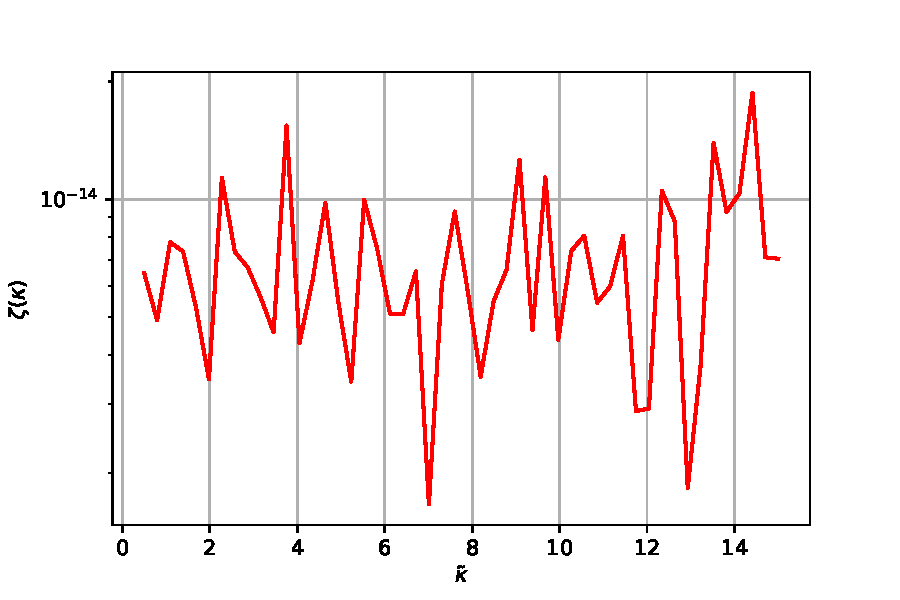
\includegraphics[width=0.5\textwidth]{validate_sol_c_i1.0c_o3.0N_30plotRangeStart_0.5plotRangeEnd_15.0.pdf}
    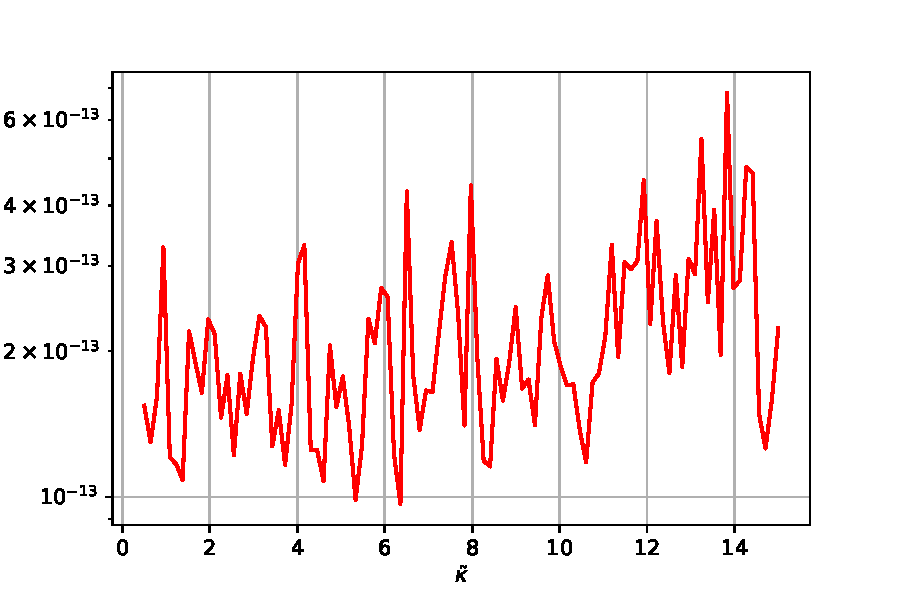
\includegraphics[width=0.5\textwidth]{validate_p_c_i3.0c_o1.0N_100plotRangeStart_0.5plotRangeEnd_15.0.pdf}
    \caption{Maximum relative residuum of the numerical solution $\zeta$ by wave number. 
    On the left plot we have $c_i = 1, c_o = 3$
    and on the right plot we have $c_i = 3, c_o = 1$. The number of considered Fourier modes is $N = 30$.}
    \label{fig:sol_validation}
\end{figure}
\noindent
As seen in fig. \ref{fig:sol_validation}, the $\zeta$-number is negligible across all values of $\kappa$ and $n$ as deviations from $0$ are in the magnitude of computer precision. This validates our derivation of $A_n^{num}$ and $w_n^{num}$.
\subsection{Projector Properties}
\label{subsection:projector_properties}
We validate our matrix $A$ with another method. We must have \(p=0\), if \((U, \theta)\) solves the problem according to P. Meury \cite{meury2007stable}. 
We can use the remark to validate that our derived matrix $A^{num}_n$ is correct.  We can formulate the property $p = 0$ with regards to $A^{num}_n$. 
Let $V_{{b}} := span( {x}_1, {x}_2)$. 
Then $p = 0$ means that for ${b} \in V_{{b}}$, every solution of  $A_n^{num} {x} = {b}_n$ satisfies $x_3 = 0$. Now let
$P_{V_{{b}}}$ be the projector onto $V_{{b}}$ and $P_3$ be the projector onto $(0, 0, 1)$.
Then $$P_3A_n^{-1}P_{V_{{b}}} = 0$$. \\
We calculate the euclidian norm of $P_3 (A^{num}_n)^{-1}P_{V_{{b}}}$ for a range of $\kappa$ values to validate this.
\begin{figure}
    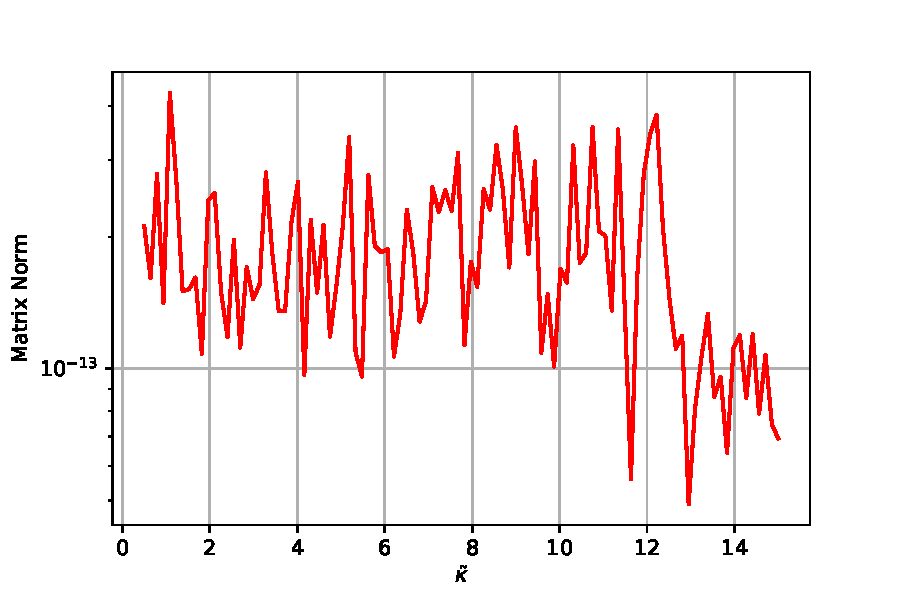
\includegraphics[width=0.5\textwidth]{validate_p_c_i1.0c_o3.0N_100plotRangeStart_0.5plotRangeEnd_15.0.pdf}
    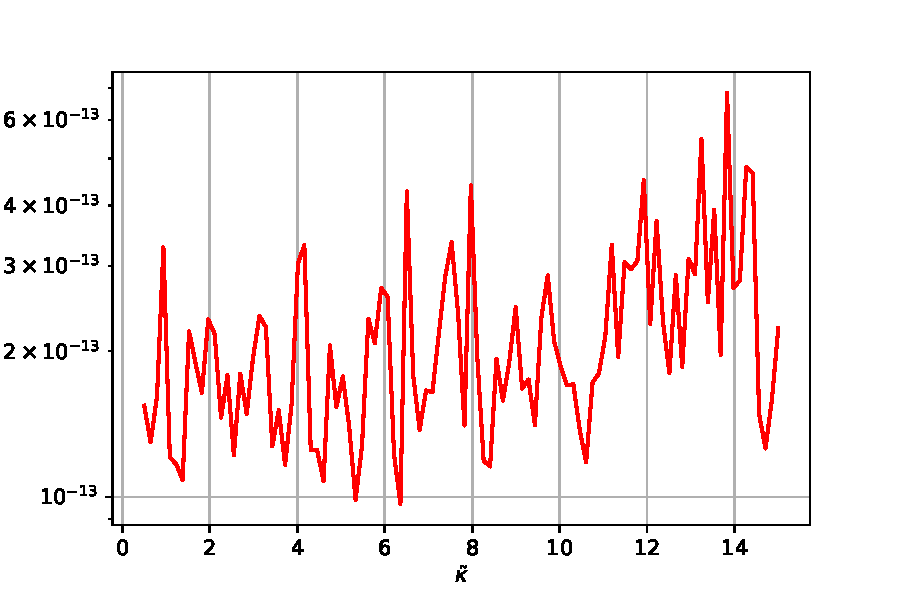
\includegraphics[width=0.5\textwidth]{validate_p_c_i3.0c_o1.0N_100plotRangeStart_0.5plotRangeEnd_15.0.pdf}
    \caption{Euclidian matrix norm of composed matrix  $P_3 (A^{num}_n)^{-1}P_{V_{{b}}}$. 
    On the left plot we have $c_i = 1, c_o = 3$
    and on the right plot we have $c_i = 3, c_o = 1$. The number of considered Fourier modes was $N = 100$.
    }
   \label{fig:p_validation}
\end{figure}
\noindent
As shown in fig. \ref{fig:p_validation}, $p = 0$ is satisfied by our operator matrix. This is another validation of our matrix $A_n^{num}$. 



\section{Numerical Results} 
\label{section:numerical_results}
Now, we numerically investigate the operator norm of the inverse operator $A^{-1}$. As established in section \ref{section:spectral_discretisation}, we can compute the inverse of the smallest singular value of $\mathrm{diag}((A_n^{num})_{n = -N}^N)$ for this operator.
\begin{figure}
    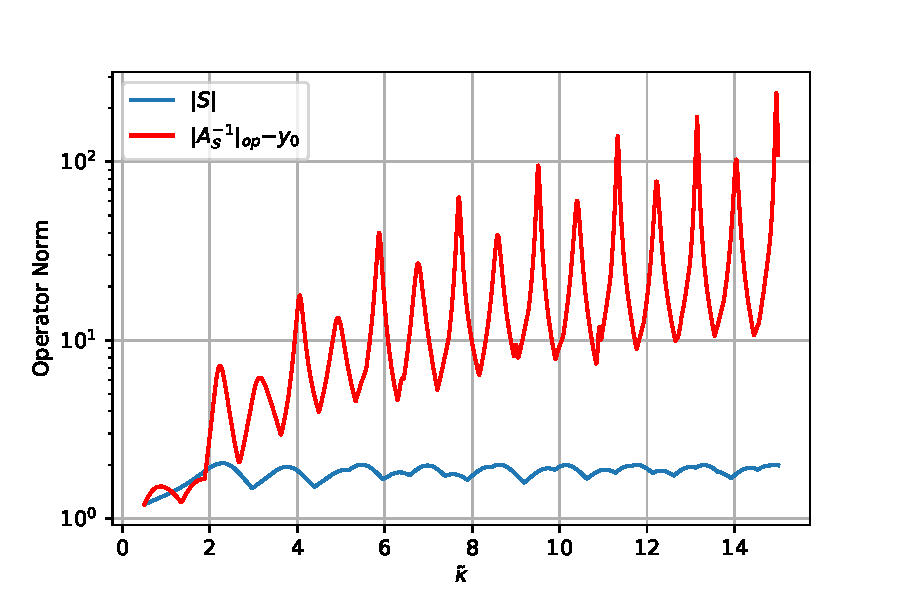
\includegraphics[width=0.5\textwidth]{simulation_scenario_1indexrange_-18.0-0.0_y_0_0.6300477177912973.pdf}
    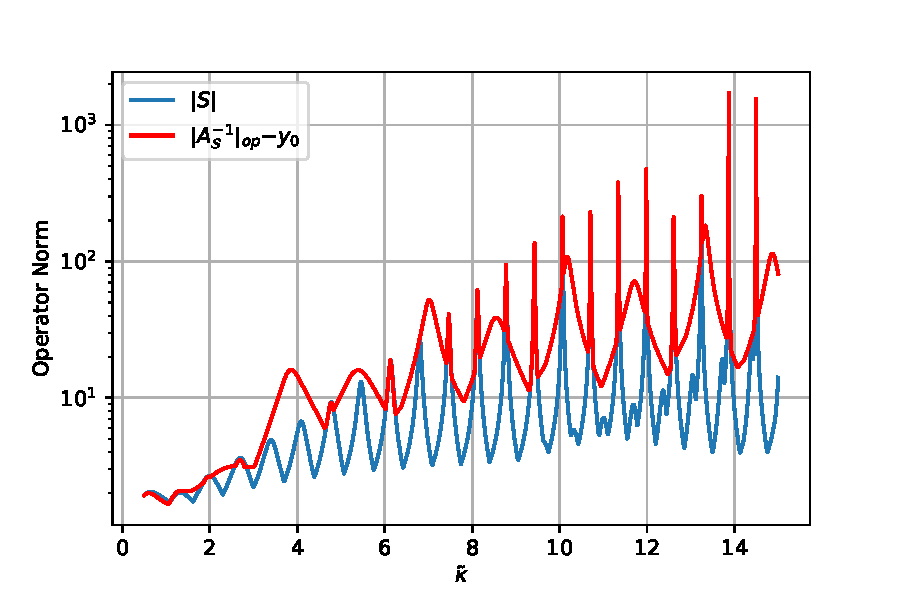
\includegraphics[width=0.5\textwidth]{simulation_scenario_2indexrange_-21.0-0.0_y_0_0.36642407845221814.pdf}
    \caption{Inverted minimum singular value $\left\|A_{\mathcal{S}}^{-1}\right\|_{o p} =\frac{1}{\sigma_{\min }(M)}$of the matrix $M = \mathrm{diag}((A_n^{num})_{n = -N}^N)$ by wave number $\kappa$. Only the first 30 Fourier blocks were considered, as the operator norms were not affected by higher modes. In fact, the highest selected mode was $n = 18$ for the left and $n =21$ for the right plot.
    When plotting the operator norm against $N$ for a fixed $\kappa$, we see that it approaches a constant value for big $N$, justifying the cutoff of $N = 30$. A more detailed explanation is given in the section \nameref{section:appendix}.
    Each of plots is shifted by an absolute value $y_0$ to allow for better comparison with the solution operator.
    In the left plot we have $c_i = 1, c_o = 3$, and $y_0 = 0.630$
    and on the right plot we have $c_i = 3, c_o = 1$, and $y_0 = 0.366$. }
   \label{fig:simulation_results}
\end{figure}
\noindent
The results of the simulation are presented in fig. \ref{fig:simulation_results}  alongside the results for the maximum euclidean norm of the solution operator.\footnote{We picked particular representative cases. More cases are shown in the \nameref{section:appendix}.} A derivation of the solution operator is provided in the \nameref{section:appendix}. \\
The solution operator exposes resonance frequencies for the case $c_i = 3, c_o =1$, called  quasi-resonances  in \cite{hiptmair2021spurious}. This resonance behavior is expected physically: If $c_i > c_o$, total internal reflection can undergo. For certain angles of internal reflection, the solution becomes very localised around the boundary $\Gamma$, meaning that the solution operator norm peaks. As we see, peaks in the solution operators coincide with the peaks of the considered inverse boundary integral operator. As we see in the right plot of fig. \ref{fig:simulation_results}, however, there are also nonphysical secondary resonances of lower frequency in $\|A^{-1}\|_{op}$. As their peaks are of similar or smaller magnitude than the primary high-frequency oscillations, the effect on the condition of the variational problem is unproblematic. Curiously, if we modify the operator $A$ such that its last row is scaled by a factor $M \gg 1$, these secondary resonances disappear.\footnote{This modification is allowed as this modified operator formulation is equivalent to the former one if we scale the last component of $w$ by $M$ too.} An example of this with $M = 30$ is shown in fig.  \ref{fig:scaled_third_equation}. At this point, a rigorous explanation of this phenomenon was not found. 

\begin{figure}
    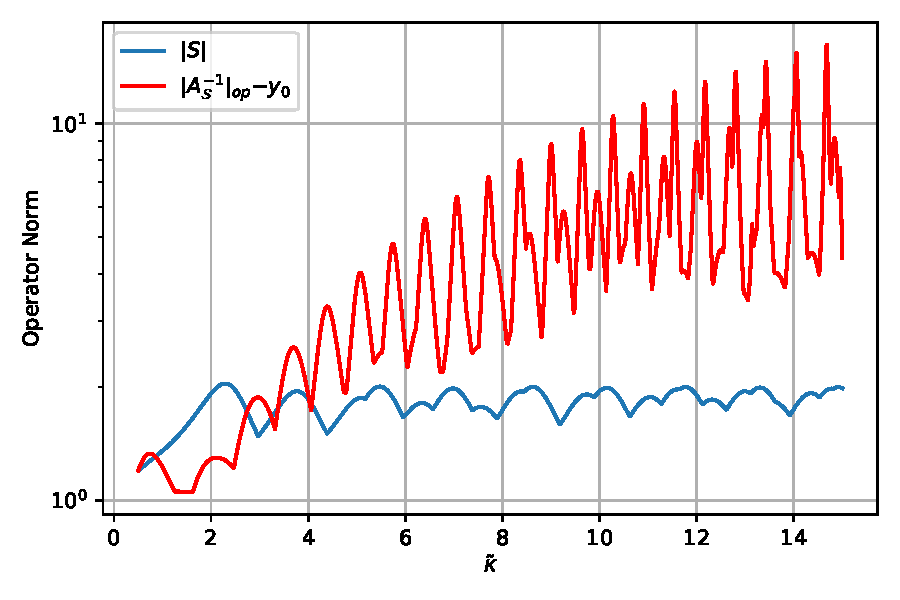
\includegraphics[width=0.5\textwidth]{simulation_scenario_13indexrange_-30.0-0.0_y_0_0.5643627199145966.pdf}
    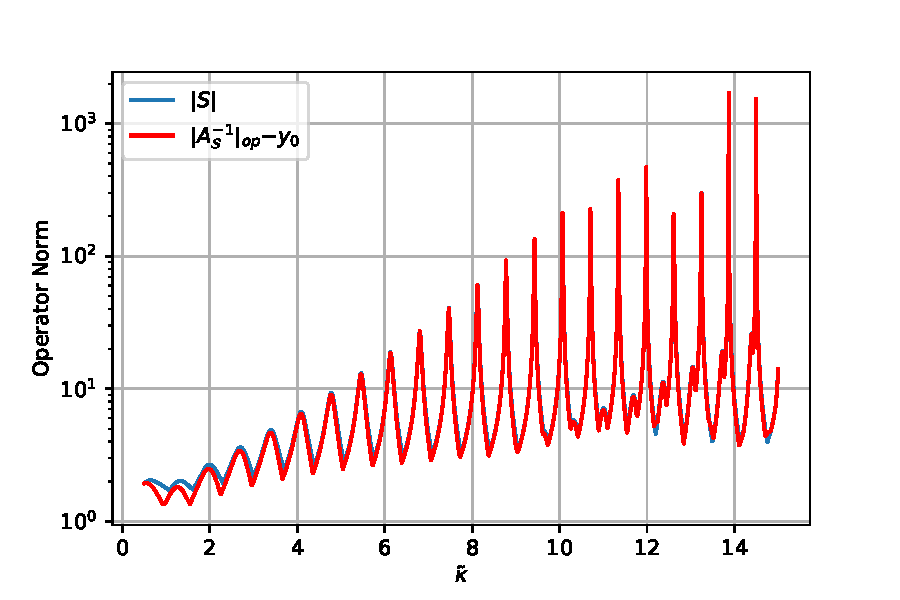
\includegraphics[width=0.5\textwidth]{simulation_scenario_12indexrange_-22.0-0.0_y_0_0.28667109315776407.pdf} 
    \caption{Inverted minimum singular value $\left\|A_{\mathcal{S}}^{-1}\right\|$ by wave number $\kappa$. In both plots, the operator $A$ is considered with the modification that its last row is scaled by a factor of $M = 30$.
    In the left plot, we have $c_i = 1.0$ and $c_o = 3.0$. In the right plot, we have $c_i = 3.0$ and $c_o = 1.0$.}
    
   \label{fig:scaled_third_equation}
\end{figure}

\noindent In the case $c_i = 1, c_o = 3$ (left plot in fig. \ref{fig:simulation_results}) the operator $A^{-1}$ exposes bad condition for some frequencies while the solution operator is regular for all frequencies. This shows that spurious quasi-resonances also occur for the regularised variational formulation. The following proposition helps explain this irregular behavior.
\newpage
\begin{proposition}
Define
    $\mathcal{L}: \mathcal{H}_{\tilde \kappa}^{\frac{1}{2}} \times \mathcal{H}_{\tilde \kappa}^{-\frac{1}{2}} \rightarrow \mathcal{H}_{\tilde \kappa}^{\frac{1}{2}} \times \mathcal{H}_{\tilde \kappa}^{-\frac{1}{2}} \times \mathcal{H}_{\tilde \kappa}^{1}$ as the map that maps the boundary conditions of eq. \ref{eq:helmholtz} to the right hand side of eq. \ref{eq:operator_formulation}
    $$
        \mathcal{L} = 
        \begin{pmatrix}
            -P_{-1}W_{\kappa} & -P_{-1} \\
            P_{1}(K_{\kappa} - \frac{1}{2}) & 0 \\
            P_{-2}W_{\kappa} & 0 \\
        \end{pmatrix}
    $$
and let
 ${E}: \mathcal{H}_{\tilde{\kappa}}^{\frac{1}{2}} \times \mathcal{H}_{\tilde{\kappa}}^{-\frac{1}{2}} \times \mathcal{H}_{\tilde{\kappa}}^{1} \rightarrow \mathcal{H}_{\tilde{\kappa}}^{\frac{1}{2}} \times \mathcal{H}_{\tilde{\kappa}}^{-\frac{1}{2}}, {E} = \begin{pmatrix}
    1 & 0 & 0 \\
    0 & 1 & 0 
\end{pmatrix}$.
    Then we can write the solution operator (see definition \ref{def:solution_operator}) as 
    $S = 
    {E}
    A^{-1} \mathcal{L}
    $.
\end{proposition}
\begin{proof}
    Consider the boundary data $f \in \mathcal{H}_{\tilde \kappa}^{\frac{1}{2}} \times \mathcal{H}_{\tilde \kappa}^{-\frac{1}{2}}$. Then by construction we have that the right hand side of eq. \ref{eq:operator_formulation} is $w = \mathcal{L} f$. Applying $A^{-1}$ to the same equation and projecting onto the first two components yields $\begin{pmatrix} U \\ \theta  \end{pmatrix} = {E}A^{-1} \mathcal{L}$. This concludes the proof.
\end{proof}  \noindent
This relationship between $A$ and $S$ implies that the lack of  $\mathcal{L}$ causes the different resonance behavior between $A$ and $S$. To show this, we lift the irregularity by introducing the operator $\mathcal{L}_\varepsilon$ for $\varepsilon > 0$: 
\begin{equation} 
\label{eq:L_operator}
\mathcal{L}_\varepsilon: \mathcal{H}_{\tilde \kappa}^{\frac{1}{2}} \times \mathcal{H}_{\tilde \kappa}^{-\frac{1}{2}} \times \mathcal{H}_{\tilde \kappa}^{1} \rightarrow \mathcal{H}_{\tilde \kappa}^{\frac{1}{2}} \times \mathcal{H}_{\tilde \kappa}^{-\frac{1}{2}} \times \mathcal{H}_{\tilde \kappa}^{1}, \quad
\mathcal{L}_\varepsilon = 
        \begin{pmatrix}
             -P_{-1}W_{\kappa}& -P_{-1} &  0\\
             P_{1}(K_{\kappa} - \frac{1}{2}) & 0 & 0 \\
             P_{-2}W_{\kappa} & 0& \varepsilon P_{-2}  \\
        \end{pmatrix}.
\end{equation}
Here we introduced the parameter $\varepsilon$ as a new formal boundary condition parameter, allowing us to invert the operator.
Assume that $\mathcal{L}_\varepsilon$ is invertible and consider the operator $$\mathcal{L}_\varepsilon^{-1}A:  \mathcal{H}_{\tilde \kappa}^{\frac{1}{2}} \times \mathcal{H}_{\tilde \kappa}^{-\frac{1}{2}} \times \mathcal{H}_{\tilde \kappa}^{1} \rightarrow  \mathcal{H}_{\tilde \kappa}^{\frac{1}{2}} \times \mathcal{H}_{\tilde \kappa}^{-\frac{1}{2}} \times \mathcal{H}_{\tilde \kappa}^{1}.$$ Note that while we introduced an additional boundary condition parameter in the third argument, it is strongly suppressed by $\varepsilon$. We will use $\varepsilon = 0.01$ in the following calculations. 
Invertibility is satisfied for the considered case of $\Gamma$, as $\mathcal{L}_\varepsilon$ becomes a blockdiagonal operator in the Fourier basis with non-vanishing determinant in each block. 
\begin{figure}
    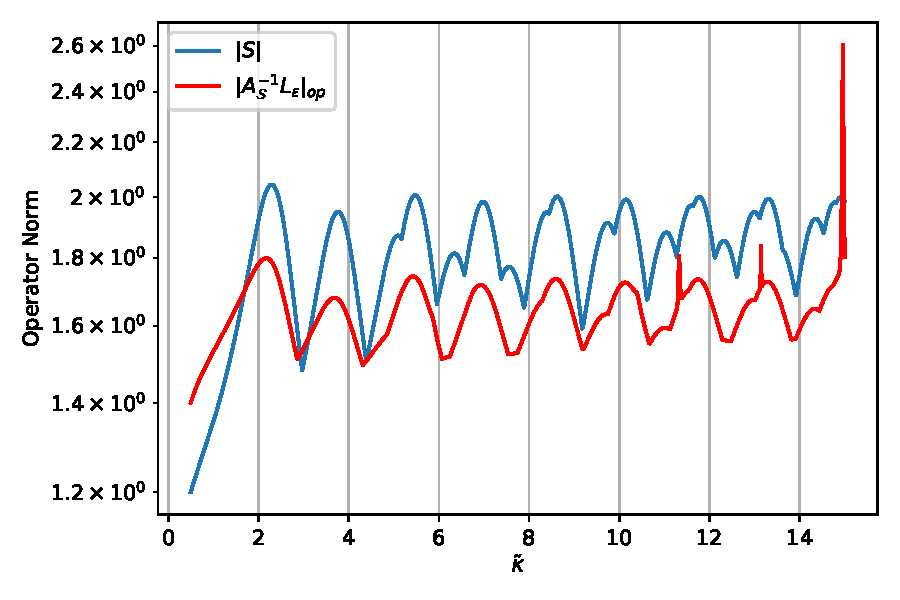
\includegraphics[width=0.5\textwidth]{simulation_scenario_10indexrange_-15.0-0.0_y_0_0.pdf}
    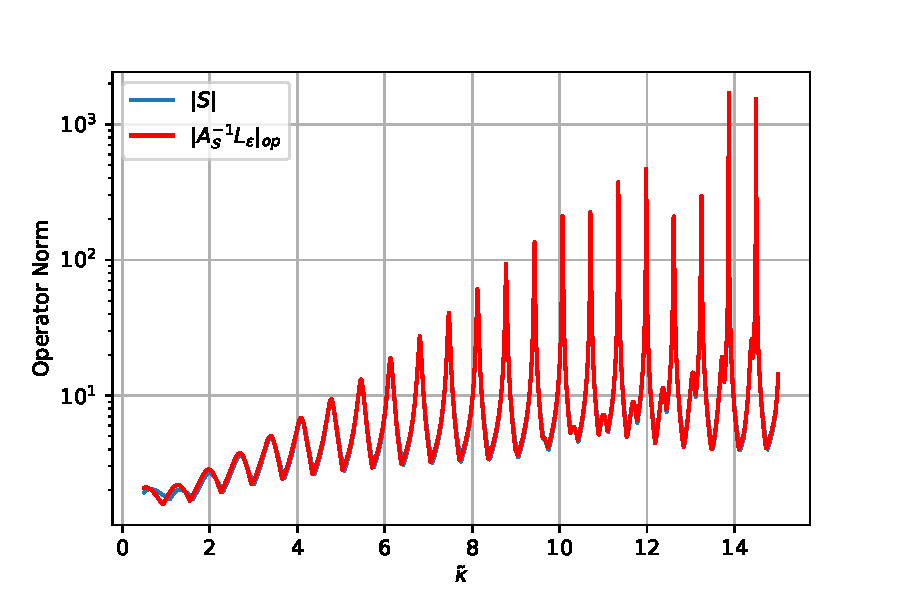
\includegraphics[width=0.5\textwidth]{simulation_scenario_11indexrange_-22.0-0.0_y_0_0.pdf}
    \caption{Inverted minimum singular value $\left\|A_{\mathcal{S}}^{-1}\mathcal{L}_\varepsilon\right\|_{o p} =\frac{1}{\sigma_{\min }(M)}$ by wave number $\kappa$. The highest selected mode out of the considered first $N = 30$ modes was $n = 15$ for the left and $n =22$ for the right plot.
    In the left plot we have $c_i = 1$ and $c_o = 3$
    and on the right plot we have $c_i = 3$ and $c_o = 1$. }
   \label{fig:regularised_results}
\end{figure}
\noindent
As the left plot of fig. \ref{fig:regularised_results} shows, the irregular resonance  behavior is indeed removed in the case $c_i < c_o$. Moreover, the right plot shows that in the case $c_i> c_o$ the secondary resonances are also removed. This implies that the spurious quasi-resonances of the considered regularised formulation operator in eq. \ref{eq:operator_formulation} were caused by the operator applied to the boundary data on the right hand side of the problem. \\
However, we did not prove the invertibility of $\mathcal{L}_\varepsilon$ for general $\Omega^-$. In particular, we did not provide an explicit expression for this inverse.\footnote{While a formal inverse (treating the entries of $\mathcal{L}_\varepsilon$ as matrix entries) can be computed symbolically, expressions in the symbolic results may not be well-defined.} Future investigations into this area could include other augmentations of the considered operator that remove these spurious quasi-resonances while also being explicitly expressed for general bounded Lipschitz domains $\Omega^- \subset \mathbb{R}^d$. 


\section{Conclusion}
This report considers a regularised variational formulation of the Helmholtz transmission problem on a two-dimensional disk (eq. \ref{eq:helmholtz}). We converted this variational formulation to an operator formulation (eq. \ref{eq:operator_formulation}). After discretizing this formulation (eq. \ref{eq:galerkin_matrix}), we calculated the inverse operator norm of the considered operator $A$ (left side operator of eq. \ref{eq:operator_formulation}) numerically. As this value is equal to the inf-sup constant of the variational problem (see section \ref{section:solvability}), this estimates the well-posedness of the variational formulation. We found, that for optical indices $c_i > c_o$ the operator introduced non-physical secondary low-frequency oscillations with small amplitude which could be surpressed by scaling up the third equation of the variational problem (fig. \ref{fig:scaled_third_equation}). A rigorous explanation for this observation was not given and may be investigated in the future.  
In the case, $c_i < c_o$ the operator exposed unphysical spurious quasi-resonances and growth behavior that the solution operator did not (fig. \ref{fig:simulation_results}). By composing with another operator $\mathcal{L}_\varepsilon^{-1}$ (eq. \ref{eq:L_operator}), we were able to remove these spurious quasi-resonances for $c_i < c_o$ and the secondary oscillations for $c_i > c_o$. Moreover, this explained the origin of spurious quasi-resonances by relating the domain of $A^{-1}$ and the solution operator $S$. However, augmentation techniques for more general geometries are required as the considered operator $\mathcal{L}_\varepsilon$ was not proven to be invertible generally, and no explicit inverse was derived for it. 

\section{Appendix}
\label{section:appendix}
\subsection{Numerical Results for other examples}
\begin{figure}
    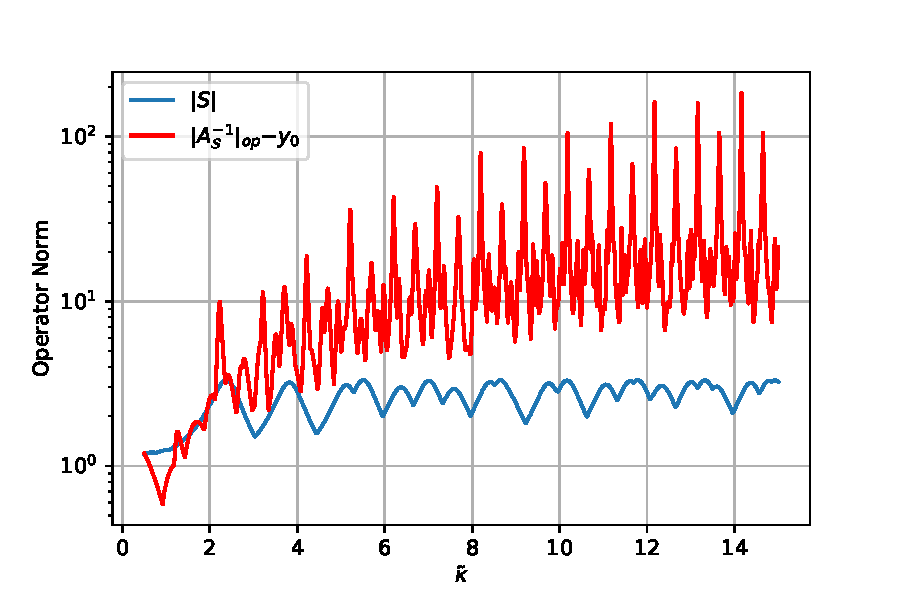
\includegraphics[width=0.5\textwidth]{simulation_scenario_3indexrange_-30.0-0.0_y_0_1.1849871455878584.pdf}
    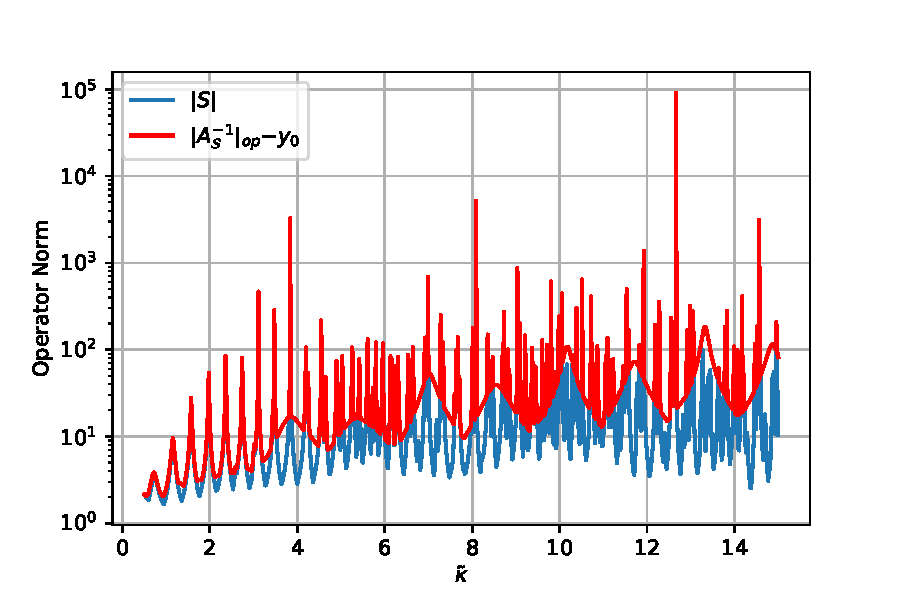
\includegraphics[width=0.5\textwidth]{simulation_scenario_4indexrange_-30.0-0.0_y_0_-0.2657606786884559.pdf} 
    \caption{Inverted minimum singular value $\left\|A_{\mathcal{S}}^{-1}\right\|$ by wave number $\kappa$. 
    In the upper left plot we have $c_i = 1$ and $c_o = 10$
    and on the upper right plot we have $c_i = 10$ and $c_o = 1$. In both plots we have $\eta = 1$.}
   \label{fig:c_other_results}
\end{figure}
\noindent
We considered the example $c_i = 1$, $c_o = 3$ and vice versa in section \ref{section:numerical_results}. In fig. \ref{fig:c_other_results} we present other examples for the refractive indices, showing that the overall trends and occurrence of spurious quasi-resonances is very similar to the considered example. \\
\begin{figure}
    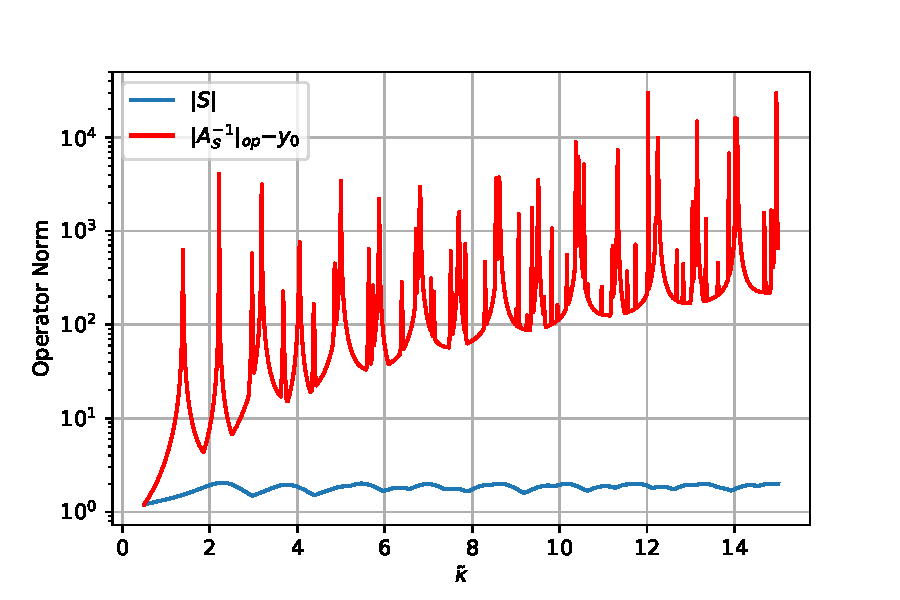
\includegraphics[width=0.5\textwidth]{simulation_scenario_8indexrange_-15.0-0.0_y_0_0.657269862562512.pdf}
    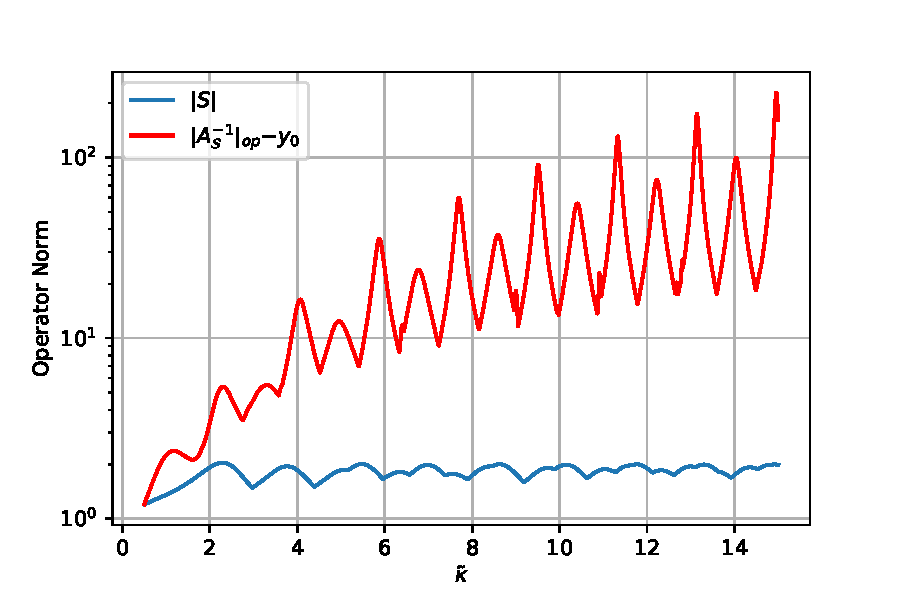
\includegraphics[width=0.5\textwidth]{simulation_scenario_9indexrange_-18.0-0.0_y_0_0.6496359740372837.pdf}  \\
    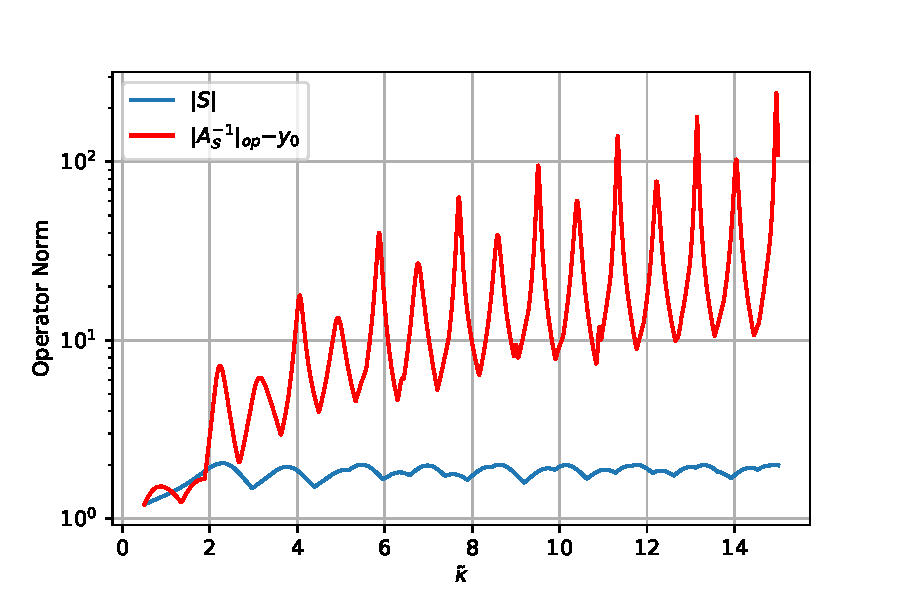
\includegraphics[width=0.5\textwidth]{simulation_scenario_1indexrange_-18.0-0.0_y_0_0.6300477177912973.pdf} 
    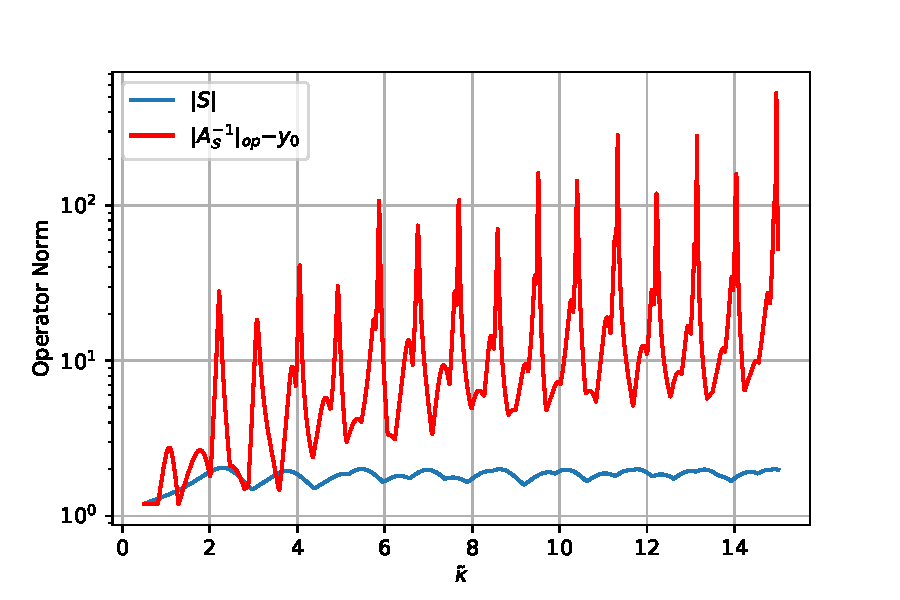
\includegraphics[width=0.5\textwidth]{simulation_scenario_7indexrange_-7.0-0.0_y_0_1.6318610980121495.pdf}  \\
     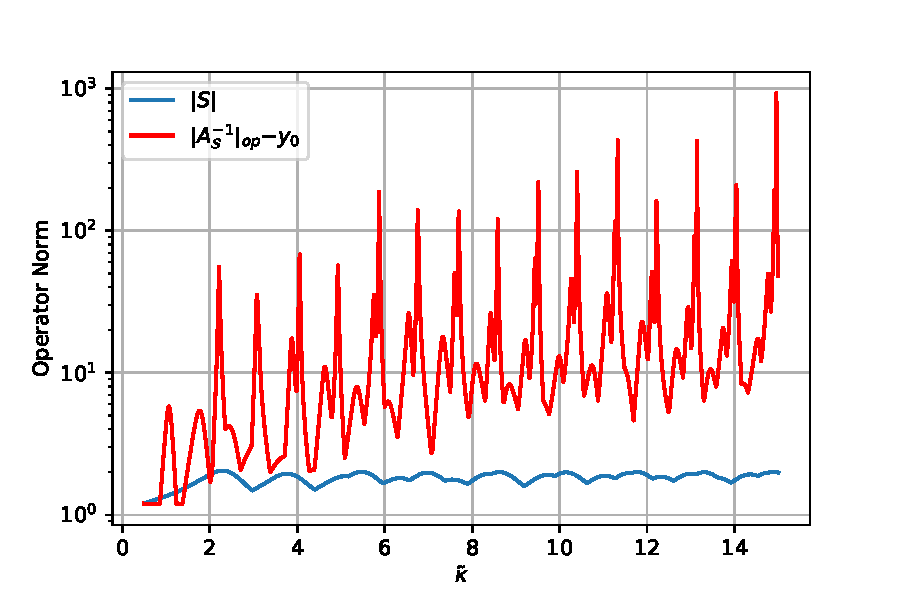
\includegraphics[width=0.5\textwidth]{simulation_scenario_6indexrange_-12.0-0.0_y_0_2.579539681123669.pdf} 
    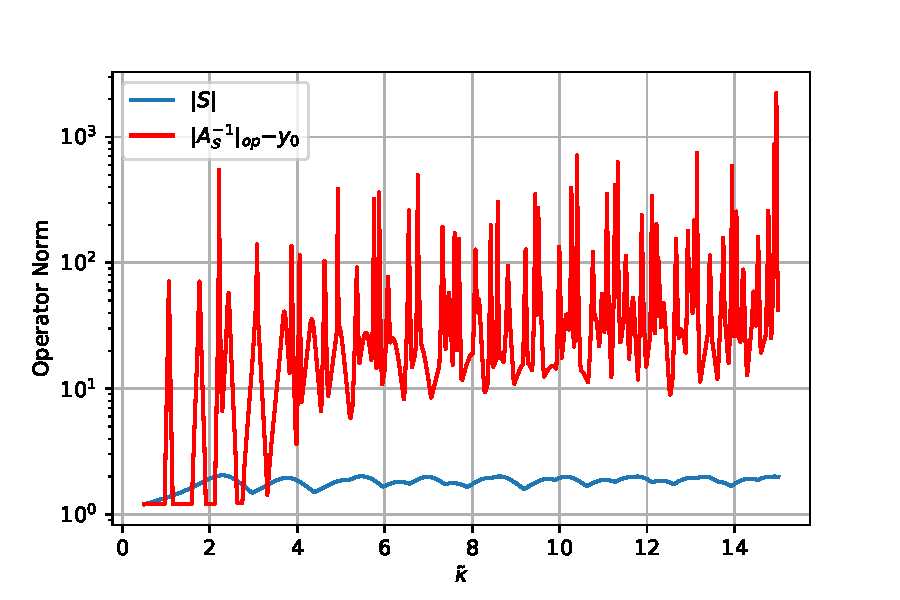
\includegraphics[width=0.5\textwidth]{simulation_scenario_5indexrange_-30.0-0.0_y_0_7.117865219377693.pdf} 
    \caption{Inverted minimum singular value $\left\|A_{\mathcal{S}}^{-1}\right\|$ by wave number $\kappa$. In all six scenarios we have $c_i = 1.0, c_o = 3.0$ and we vary $\eta$. The values of $\eta$ are as follows. Top left: $\eta = 0$, top right: $\eta = 0.5$, middle left: $\eta = 1.0$, middle right: $\eta = 5.0$,  lower left: $\eta = 10.0$, and lower right: $\eta = 100.0$.}
     \label{fig:eta_other_results}
\end{figure}
\noindent Moreover, we only studied $\eta = 1.0$ in section \ref{section:numerical_results}. As shown in fig. \ref{fig:eta_other_results}, the operator growth is smallest in the range from $\eta = 0.5$ to $\eta = 1.0$ out of the selected values. This is in agreement with the results of P. Meury's doctoral thesis, where he achieved optimal stability around $\eta = 1.0$ \cite{meury2007stable}.
\\
Lastly, we will justify the introduction of a cutoff $N$ for the Fourier modes. In fig. \ref{fig:convergence_test} the singular value of the operator block $A^{num}_n$ inverse are plotted as a function of the mode $n$. We clearly see, that for $n$ big enough the singular value converges. 
\begin{figure}
\center{
    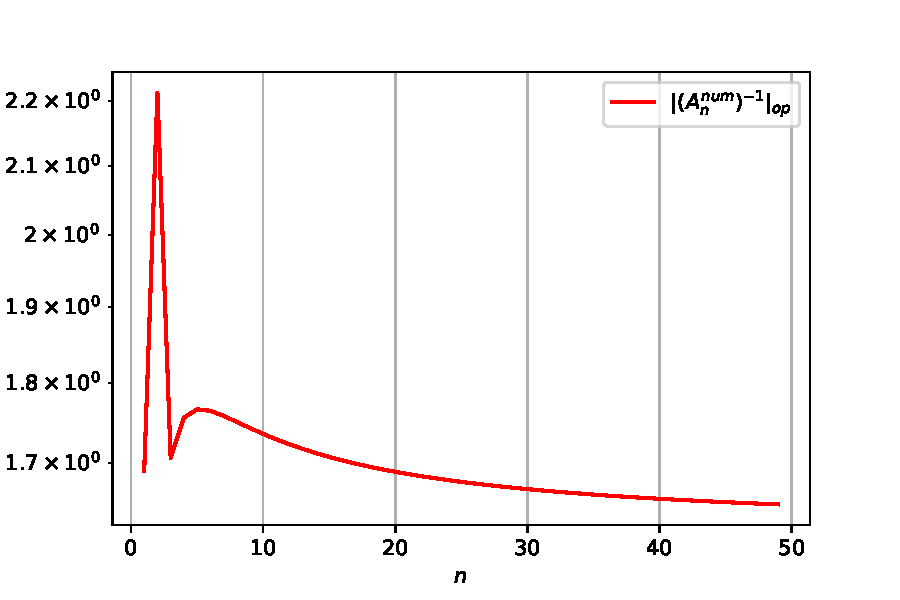
\includegraphics[width=0.5\textwidth]{convergenceTest_c_i1.0c_o_1.0kappa_1.0.pdf}
    \caption{Inverted singular value $\left\|A^{num}_n\right\|$ for fixed $\kappa$ as a function of the Fourier mode $n$. }}
\end{figure}
\label{fig:convergence_test}
\noindent
There is also a simple theoretical explanation to justify the cutoff in $n$: consider the matrix $A^{num}_n$ as defined in eq. \ref{eq:galerkin_matrix}. We have the approximate form \(J_{n}(x) \sim \frac{1}{\Gamma(n+1)}\left(\frac{x}{2}\right)^{n}\) for \(x \ll \sqrt{n+1}\) \cite{abramowitz1972abramowitz}. This implies that $\lim\limits_{n \rightarrow \infty}\frac{\alpha_n}{n} = 1$.
Moreover, we know that $\beta_n = O(n^2)$. The following limits can be validated numerically or symbolically:\footnote{Note that the $n$-dependence is not written out explicitly.}
\begin{align}
    \lim\limits_{n \rightarrow \infty} \lambda^{(V)} = \frac{1}{2} \nonumber \\
    \lim\limits_{n \rightarrow \infty} \lambda^{(K)} = 0 \nonumber \\
    \lim\limits_{n \rightarrow \infty} \frac{\lambda^{(W)}}{n} = \frac{1}{2}. \nonumber
\end{align} Therefore, the matrix $A^{num}_n$ behaves the following for big $n$:
$$
    A^{num}_n {\sim} 
    \begin{pmatrix}
        1 + \frac{1}{2} & - \frac{1}{2} & 0 \\
        \frac{1}{2} & \frac{1}{2} & i \overline{\eta} \\
        - \frac{1}{2} & -\frac{1}{2} & O(n)
    \end{pmatrix} \text { for } n \rightarrow \infty.
$$
 The smallest singular value of this matrix is given by $\inf\limits_{|x| = 1} \|A^{num}_n x\| $. Since one of the entries in the third column has order $n$, The extremal value of $x$ must have the form $(x^1_n, x^2_n, 0)$. However, the matrix in the first two columns converges, implying convergence of the minimal singular value.

\subsection{Constructing the Solution Operator}
Plugging the Fourier ansatz into eq. \ref{eq:helmholtz} and imposing convergence at the origin and 
the Sommerfeld radiation condition results in
\begin{align}
    u^- = \sum\limits_{n = -\infty}^\infty u_n^- \frac{J_n(\sqrt{ c_i} \tilde \kappa r)}{J_n(\sqrt{ c_i} \tilde \kappa)} e^{i n \phi} \nonumber \\
    u^+ = \sum\limits_{n = -\infty}^\infty u_n^+ \frac{H_n(\sqrt{ c_o} \tilde \kappa r)}{H_n(\sqrt{ c_o} \tilde \kappa)} e^{i n \phi} \nonumber
\end{align}
where $u_n^-$ and $u_n^+$ are the restrictions of $u$ to $\Omega^-$ und $\Omega^+$.\\
Extend $f^i = \sum\limits_{n = -\infty}^\infty f^i_n e^{in\phi}$ for $i=1,2$. The transmission condition $\gamma_{C}^{+} u^{+}=\gamma_{C}^{-} u^{-}+f$ implies 
\begin{align}
    \begin{pmatrix}
        1 & -1 \\
        \sqrt{c_i} \tilde \kappa \frac{J_n^\prime(\sqrt{c_i} \tilde \kappa)}{J_n(\sqrt{c_i} \tilde \kappa)} & 
        -  \sqrt{c_o} \tilde \kappa \frac{H_n^\prime(\sqrt{c_o} \tilde \kappa)}{H_n(\sqrt{c_o} \tilde \kappa)}
    \end{pmatrix} 
    \begin{pmatrix}
        u_n^- \\u_n^+
    \end{pmatrix}
    = 
    \begin{pmatrix}
        f_n^1 \\ f_n^2
    \end{pmatrix}.
\end{align} 
By using the well-known inverse of a 2x2 matrix we obtain 
\begin{equation}
    u_n^- = \zeta(-\sqrt{c_o}\tilde \kappa J_n(\sqrt{c_i} \tilde \kappa) H_n^\prime(\sqrt{c_i} \tilde \kappa)f_n^1 
    + J_n(\sqrt{c_i} \tilde \kappa) H_n(\sqrt{c_o} \tilde \kappa) f_n^2).
\end{equation}
where $\zeta := \frac{1}{\sqrt{c_i} \tilde \kappa J_n^\prime(\sqrt{c_i} \tilde \kappa) H_n(\sqrt{c_o} \tilde \kappa)
-\sqrt{c_o} \tilde \kappa H_n^\prime(\sqrt{c_o}\tilde \kappa) J_n(\sqrt{c_i} \tilde \kappa)
}$.
This presents the solution operator, as we get $\gamma_D^-$ from restriction to the boundary.
$\gamma_N^-$ can be directly obtained by restriction of the normal derivative of $u_n^-$ to the boundary 
which is equivalent to multiplying the Fourier coefficients by $\sqrt{c_i} \tilde \kappa\frac{J_n^\prime(\sqrt{c_i}\tilde \kappa)}{J_n(\sqrt{c_i}\tilde \kappa)}$.
After rescaling the $u_n$, $f_i^n$ to the complete orthonormal system defined in eq. \ref{eq:basis},
we obtain the solution operator matrix: 
\begin{equation}
    S_{io}^n = 
    \zeta
    \begin{pmatrix}
        -\sqrt{c_o}\tilde \kappa J_n(\sqrt{c_i} \tilde \kappa) H_n^\prime(\sqrt{c_i} \tilde \kappa) & 
        \sqrt{n^2 + \tilde \kappa^2} J_n(\sqrt{c_i} \tilde \kappa) H_n(\sqrt{c_o} \tilde \kappa)  \\
        -\frac{1}{\sqrt{n^2 + \tilde \kappa^2}}\sqrt{c_o}\sqrt{c_i} \tilde \kappa^2 J^\prime_n(\sqrt{c_i} \tilde \kappa) H_n^\prime(\sqrt{c_i} \tilde \kappa) & 
        \sqrt{c_i} \tilde \kappa J^\prime_n(\sqrt{c_i} \tilde \kappa) H_n(\sqrt{c_o} \tilde \kappa) \\
    \end{pmatrix}
\end{equation}
\noindent
that maps the Fourier coefficients of $f$ in the complete orthonormal system for $\mathcal{H}^{\frac{1}{2}}\times \mathcal{H}^{-\frac{1}{2}}$
 to the Fouier coefficients of $\gamma_C^-u$ in the same basis.

\subsection{Proof of Theorem \ref{thm:variational_perspective}}
\begin{proof}[Proof of Theorem \ref{thm:variational_perspective}]
    Consider the operator problem $Au = w$ with linear operator $A$ as defined in Lemma \ref{lem:operator_formulation}.
    $A$ is bounded as continuity of the sesquilinear form implies that there is a constant $M>0$ such that
    $$
        \|A u\|_{H}^{2}=(A u, A u)_{H}=|{a(u, A u)}| \leq M\|u\|_{H}\|A u\|_{H}
    $$
    Moreover $A$ is injective: assume $Au = 0$ for some $u \in H \backslash \{0\}$. Then $|(Au, v)_H| =0 \text{ } \forall v \in H$. In particular, $\sup\limits_{v\in H} |(Au, v)_H| = 0$. However,
    $$
        0 = \sup\limits_{v\in H \backslash \{0\}} \frac{|(Au, v)_H|}{\|u\|_H \|v\|_H} \geq \inf\limits_{t \in H \backslash \{0\}}\sup\limits_{v\in H \backslash \{0\}} \frac{|(At, v)_H|}{\|u\|_H \|v\|_H} = \inf\limits_{t \in H \backslash \{0\}}\sup\limits_{v\in H \backslash \{0\}} \frac{|{a(t, v)}|}{\|u\|_H \|v\|_H}= \gamma
    $$
    is a contradiction as $\gamma > 0$ by assumption. Thus $u = 0$ and $A$ is injective. \\
    Now we show surjectivity of $A$. $A$ is surjective if every $v \in H$ is contained in its image.
    First, note that $\mathrm{Im}(A)$ is closed. Assume we have a Cauchy sequence $w_n$ in $\mathrm{Im}(A)$. Then there are $u_n \in H$ such that $Au_n = w_n$. We have
    $$
     \left\|u_{l}-u_{m}\right\|_{H} \leq \frac{1}{\gamma} \sup _{v \in H \backslash\{0\}} \frac{|a(u_l - u_m,v)|}{\|v\|_H} = 
    \frac{1}{\gamma} \sup_{v \in H \backslash\{0\}} \frac{|(w_l - w_m, v)_H|}{\|v\|_H} =  \frac{1}{\gamma}\|w_l - w_m\|_{H}.
    $$
    In the first equation we used the definition of $\gamma$, in the second we used that $a(u_n,v) = (Au_n, v)_H = (w_n, v)_H$  and in the third we used the Cauchy-Schwarz inequality. We showed that $u_n$ is Cauchy. $H$ is complete, so $u_n$ converges in $H$. Because of continuity of $A$, this implies that $$\lim\limits_{n\rightarrow \infty} Au_n = \lim\limits_{n\rightarrow \infty} w_n = A \lim\limits_{n \rightarrow \infty} u_n.$$ Therefore $\mathrm{Im}(A)$  is closed. 
    Since $\mathrm{Im}(A)$ is closed, we have $H = \mathrm{Im}(A) \oplus \mathrm{Im}(A)^\perp$ according to \cite{rudin1991functional}. Therefore, we just have to show that the orthogonal complement of $A$ is empty. This is the case if the map $u \mapsto (Au, v)$ is nontrivial for all $v \in H$. We prove this by contradiction. Assume there is a $v \in H$ such that $u \mapsto (Au, v)$ is the zero map. Then   $a(u, v) = 0  \text{ }\forall u \in H$, violating the C2 condition $\sup\limits_{u \in H \backslash\{0\}} \frac{|a(u, v)|}{\|u\|_{H}}>0 \text{ } \forall v \in H \backslash\{0\}$. Thus, $\mathrm{Im}(A)^\perp$ is empty and $A$ is surjective.
    \\
    % Now assume $Y$ is a proper subset of $H^*$. According to Corollary 5.4 in \cite{ovchinnikov2018functional} this implies that there is a $v \in (H^*)^*$ such that $v_{|Y} = 0$. However, this is a contradiction to C2. Since $(Au)^* \in Y$ for every $u \in H$ by definition, we have 
    % $$0 = |v((Au)^*)| = |(Au)^*(v)| = |(Au, v)_H| = |a(u, v)|.$$ In particular, then 
    % $$
    % \sup_{u \in H\backslash \{0\}}a(u, v) = 0,
    % $$
    % contradicting C2.
    % \\
    % Therefore, we must have $Y = H^*$, proving surjectivty of $A$. 
    This concludes the proof of solvability and bijectivity as $A^{-1} \tau$ is the solution operator where $\tau$ is the bijective antilinear map $\tau: H^* \rightarrow H$ from the Riesz representation theorem. \\
    The last claim about the norm of the solution operator follows directly: 
    \begin{align*}
    \|S_{var}\|_{H^* \rightarrow H} & = \sup\limits_{b \in H^*\backslash \{0\}}\frac{\|Sb\|_{H}}{\|b\|_{H^*}} = 
    \sup\limits_{b \in H\backslash \{0\}}\frac{\|Sb\|_{H}}{\sup\limits_{v\in H\backslash \{0\}} \frac{|b(v)|}{\|v\|_H}} = 
    \sup\limits_{b \in H^*\backslash \{0\}}\frac{\|u(b)\|_{H}}{\sup\limits_{v\in H\backslash \{0\}} \frac{|a(u, v)|}{\|v\|_H}} \\
    & = \sup\limits_{u \in H\backslash \{0\}}\frac{\|u\|_{H}}{\sup\limits_{v\in H\backslash \{0\}} \frac{|a(u,v)|}{\|v\|_H}} = \frac{1}{\inf\limits_{v\in H\backslash \{0\}}\sup\limits_{u \in H\backslash \{0\}}{ \frac{|a(u,v)|}{\|v\|_H\|u\|_{H}} }} = \frac{1}{\gamma}.
    \end{align*}
    Note that we used bijectivity in the fourth equation, allowing us to write $v(u)$ instead of $u(v)$ and taking the supremum over $u$. Moreover we used $b(v) = a(u,v)$ from LVP.
\end{proof}

\newpage
\section*{Symbols}

This is an index of symbols repeatedly used in this report with references where the corresponding terms are defined (if applicable).
\begin{itemize}
    \item $H^1(\Omega)$: Sobolev space, \cite{hiptmair2012numerical}.
    \item $H_{\mathrm{loc}}^{1}\left(\Omega^{\pm}\right)$:  \(H_{\text {loc }}^{1}\left(\Omega^{\pm}, \Delta\right):=\left\{v: \chi v \in H^{1}\left(\Omega^{\pm}\right), \Delta(\chi v) \in L^{2}\left(\Omega^{\pm}\right)\right.\)for all \(\left.\chi \in C_{\text {comp }}^{\infty}\left(\mathbb{R}^{d}\right)\right\}\), section \ref{section:introduction}
    \item $H^{\frac{1}{2}}(\Gamma)$: Dirichlet trace space, \cite{hiptmair2018advanced}.
    \item $H^{-\frac{1}{2}}(\Gamma)$: Neumann trace space, \cite{hiptmair2018advanced}.
    \item $\Omega^{-}$: Generally a bounded Lipschitz domain.  $\Omega^{0} = B_1(0) \subset \mathbb{R}^2$ for most of the report, section \ref{section:introduction}. 
    \item $\Omega^{+}$: \(\Omega^{+}:=\mathbb{R}^{d} \backslash \overline{\Omega^{-}}\), section \ref{section:introduction}.
    \item $\Gamma$: \(\Gamma:=\partial \Omega^{-}=\partial \Omega^{+}\).
    \item \(\operatorname{grad}_{\Gamma}\): surface gradient, \cite{sauter2010boundary}.
    \item \(\operatorname{grad}_{\Gamma}\): adjoint map of $\hat{\phi} \operatorname{grad}_{\Gamma}$, \ref{section:operator_formulation}.
    \item $\varphi^{\pm}$: \(\varphi^{\pm}:=\left.\varphi\right|_{\Omega^{\pm}}\), section \ref{section:introduction}.
    \item $C_{\text {comp }}^{\infty}\left(\mathbb{R}^{d}\right)$: Smooth functions with compact support
    \item $\gamma_{D}^{\pm}$: Dirichlet trace operators, section \ref{section:introduction}.
    \item $\gamma_{N}^{\pm}$: Neumann trace operator, section \ref{section:introduction}.
    \item \(\gamma_{C}^{\pm}\): Cauchy trace, section \ref{section:introduction}.
    \item $f$: Boundary conditions of Helmholtz transmission problem, section \ref{section:introduction}.
    \item $\kappa, \tilde \kappa$: Wave number, section \ref{section:introduction}.
    \item $c_i, c_o, \tilde c$: Refractive indices, section \ref{section:introduction}.
    \item $U, \theta, p$: Solution of Helmholtz transmission problem, section \ref{section:introduction} \& section \ref{section:regularized_variational_formulation}.
    \item $S$: Solution operator, section \ref{section:introduction}.
    \item $\mathrm{DtN}^-_\kappa$: Interior Dirichlet-to-Neumann map, section \ref{section:definitions}.
    \item $\mathrm{V}_\kappa, \mathrm{K}_\kappa, \mathrm{K}^\prime_\kappa, \mathrm{W}_\kappa$: Boundary integral operators, section \ref{section:definitions}.
    \item $q_\kappa(\cdot, \cdot), b(\cdot, \cdot)$: Bilinear forms in regularized variational formulation, section \ref{section:regularized_variational_formulation}.
    \item $g_i$: Right hand side of regularized variational formulation, section \ref{section:regularized_variational_formulation}.
    \item \(\mathcal{H}^{s}(\Gamma)_{\tilde \kappa}\): Fourier Sobolev Hilbert space, section \ref{section:operator_formulation}.
    \item $A$: Left hand side operator in the regularized operator formulation, section \ref{section:operator_formulation}.
    \item $\mathcal{B}$: Right hand side boundary value operator in the regularized operator formulation, section \ref{section:operator_formulation}.
    \item $\mathcal{S}^s_N$: Restricted Sobolev space for numerical calculations, section \ref{section:spectral_discretisation}.
    \item $\lambda^{(\mathrm{V})}, \lambda^{(\mathrm{K})}, \lambda^{(\mathrm{K}^\prime)}, \lambda^{(\mathrm{W})}$: Fourier eigenvalues of boundary value operators, section \ref{section:spectral_discretisation}.
    \item $\alpha_n, \beta_n$: Fourier eigenvalues of operators occurring in regularised operator, section \ref{section:spectral_discretisation}.
    \item $A^{num}_n$: Galerkin matrix, section \ref{section:spectral_discretisation}.
    \item \(\mathcal{L}_\varepsilon\): augmenting operator  for  $A$, section \ref{section:numerical_results}.
\end{itemize}
    
    

\section*{Code}
Calculations and plots were implemented in Python. The corresponding files are available \href{https://github.com/FredericJorgensen/spurious-quasi-resonances-coupled-variational-formulation}{here}.

\bibliography{references}
\bibliographystyle{ieeetr}

\end{document}
